\section{The preCICE library}
\label{sec:library}

In this section, we present the core library of preCICE in a nutshell. 
\autoref{fig:overview} visualizes the concept and basic functional components of preCICE.
In the figure, several types of simulation codes are coupled: computational fluid dynamics (CFD) solvers, finite-element method (FEM) solvers, in-house solvers, and particle solvers. Please note that we use these types as examples to introduce the overall concept, not as strict non-overlapping categories.
In the following, we refer to coupled simulation codes as \textit{participants} of a coupled simulation.
The glue code between a participant's code and the preCICE library is called adapter.
Depending on the participant, an adapter can be a module or a class of the participant's code or a complete stand-alone software, which uses some callback interface of the participant. 
In some cases, an adapter can also be a sophisticated script that calls the participant as well as preCICE, but such a software design contradicts the main idea behind the library approach of preCICE to some extent.
preCICE comes with several ready-to-use adapters, which are listed in the picture.
Not all adapters, though, feature the same level of maturity.
Users of preCICE can develop adapters for their own (in-house) codes by using the preCICE API, which is available in the most important languages used in Scientific Computing.
An adapter is responsible for what we call \textit{coupling physics}, meaning how to translate nodal coupling values from preCICE into boundary conditions or forcing terms and, reciprocally, how to extract nodal coupling values from internal fields to provide them to preCICE.  
If we say that an adapter can handle a certain type of coupling physics, for example conjugate-heat transfer, it basically means which type of variables, e.g., temperature or heat flux, the adapter is able to read and write.

\begin{figure}[h!]
\centering
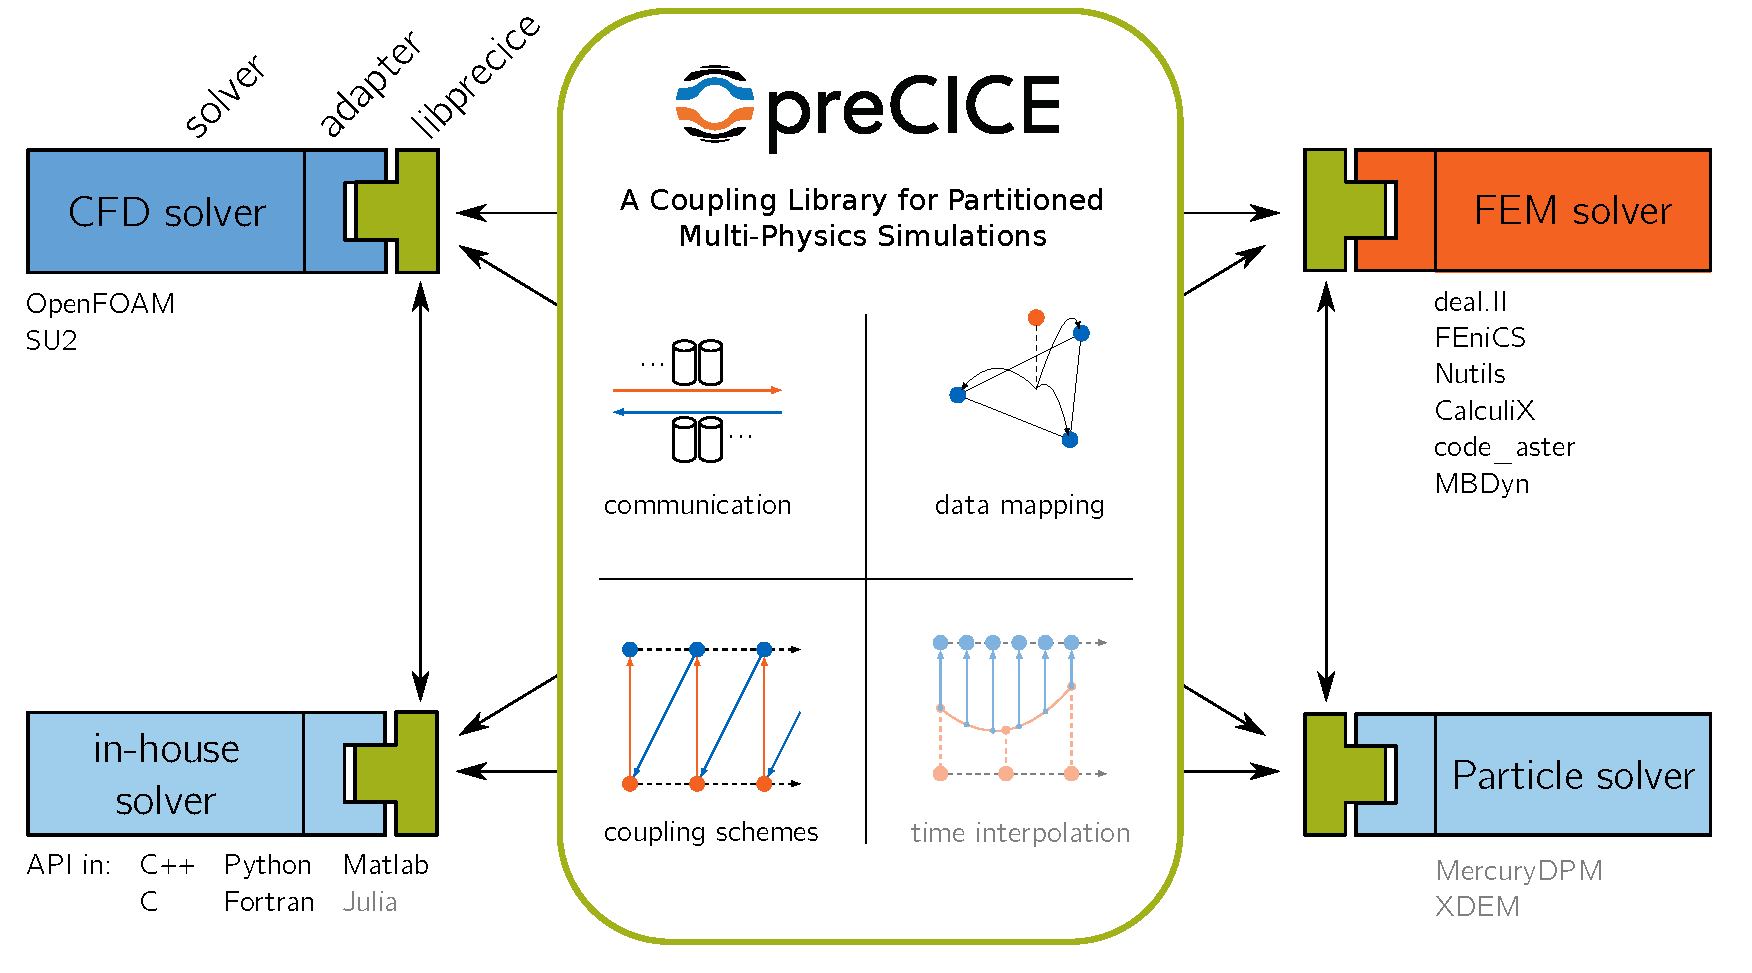
\includegraphics[width=\textwidth]{figs/precice-overview.pdf}
\caption{
\label{fig:overview} Concept and basic functional components of preCICE. Components that are work in progress and not yet released are shown grayed out.}
\end{figure}

preCICE itself has no notion of physics.
Instead, preCICE itself is responsible for the technical aspects of coupling and the coupling numerics, depicted in the middle of \autoref{fig:overview}. We now give a first brief overview of these components going from top left to bottom right:
(i) Coupled participants are separate executables, potentially running on different nodes in a heterogeneous compute cluster with independent MPI communicators.
preCICE handles the communication between these executables. 
The communication is asynchronous and completely parallel. 
Only those ranks of the participants that need to exchange coupling data communicate with each other.  
Technically, the communication is based on either MPI Ports or TCP/IP, configurable at runtime.
(ii) preCICE implements coupling schemes. Coupling schemes, on the one hand, define the logical coupling flow, i.e., which participant sends which data to which other participant and how the execution of time steps is synchronized between the participants.
On the other hand, coupling schemes comprise acceleration methods for implicit coupling such as Aitken under-relaxation or quasi-Newton methods. 
(iii) Moreover, preCICE allows to map coupling data between non-matching and non-conforming coupling meshes. 
To this end, the user can choose between projection-based methods (nearest neighbor or nearest projection) or radial-basis function interpolation.
(iv) Finally, preCICE also handles interpolation in time.
Currently, only plain sub-cycling is supported, but higher-order interpolation is under development~\cite{QNWI} and will be available in future releases.
 
Please note that, even though \autoref{fig:overview} depicts a significant green box in the middle, there is no central server-like instance running, even for parallel simulations. 
preCICE uses a pure peer-to-peer library approach.
The only executables that are started are the participants, which all call preCICE.

The current section describes the main concepts of the core library and is structured as follows. 
In \autoref{ssec:cplscheme}, \autoref{ssec:mapping}, and \autoref{ssec:com}, we describe the methods preCICE uses for coupling schemes, data mapping, and communication, respectively. Different options to get and if necessary build preCICE are listed in \autoref{ssec:building}. Finally, \autoref{ssec:api} explains the API and the runtime configuration of preCICE.

\subsection{Coupling schemes and acceleration}
\label{ssec:cplscheme}

%\textbf{Coupling Schemes.}
Coupling schemes and acceleration methods are at the very center of the preCICE core and define the coupling flow. As they have been studied in numerous publications (e.g.,~\cite{Mehl2016, Lindner2015_MVQN, Scheuf:QN}), we restrict the description to 
a short summary showcasing which combinations of coupling options and acceleration
schemes lead to robust and efficient partitioned simulations.
%
The coupling options can be configured at runtime. preCICE distinguishes: (i) \textit{uni-directional} or \textit{bi-directional} coupling, i.e., data dependencies between the participants in one direction only (example: full flow simulation coupled to an acoustic far field, where the acoustic far fields receives background velocity and pressure values as well as acoustic perturbations at the coupling interface, but we do not observe acoustic waves traveling back into the flow region) or data dependencies in both directions (e.g., fluid-structure interaction); (ii) \textit{explicit} or \textit{implicit} coupling, i.e., execution of each participant once per time step or execution of multiple iterations per time step, such that the values at the end of the time step fulfill all coupling conditions; and (iii) \textit{parallel} or \textit{serial} coupling, i.e., simultaneous
or one-after-the-other execution of participants.
%The specification of data to be exchanged is usually determined by the numerical (and physical) requirements of the concrete application at hand, such that we can not give general recommendations here\footnote{For details on data mapping between non-matching meshes, see \autoref{ssec:mapping}.}. 
%
 Uni-directional coupling requires data transfer only from one participant to the other. Thus, only an explicit coupling makes sense in this case, which can, however, be both serial or parallel. For bi-directional coupling, we have four different coupling scheme options: (i) parallel-explicit, (ii) serial-explicit, (iii) parallel-implicit, (iv) serial-implicit. We show the six different resulting coupling schemes in
 \autoref{fig:cpl_simple}.
 %
In the following, we focus on two non-trivial aspects of coupling: the coupling of more than two participants (multi-code coupling) and the choice of suitable convergence acceleration schemes for implicit coupling.

\begin{figure}[h!]
\centering
\input{figs/coupling-strategies/tikzcode.tex}
\caption{
\label{fig:cpl_simple}
Different coupling options in preCICE for two participants $S_1$ and $S_2$ defined by combinations of (i) uni-directional or bi-directional (data transfer between two participants only in one or in both directions); (ii) explicit or implicit (execution of both participants once per time step or iterative solution of a fixed-point equation); (iii) parallel or sequential (simultaneous or one-after-the-other execution of two participants). $\mathcal{A}$ symbolizes a convergence acceleration method.}
\end{figure}


\paragraph{Multi-code coupling} 
For multi-code coupling, coupling schemes can be configured in two different ways: (i) for each pair of participants separately or (ii) as an overall multi-coupling scheme. For (i), theoretically, all combinations of coupling options are possible. However, combinations of several pairwise implicit coupling schemes have been shown to be numerically unstable~\cite{Bungartz2014_MIQN_CompuMech}. Still, pairwise coupling can be the best option for some combinations of explicit and implicit coupling. One such example is the extension of the fluid-acoustics example mentioned above shown in~\cite{Lindner2020_ExaFSA}: a bi-directional, implicit, and serial coupling of a structure solver with a flow solver, combined with a uni-directional, explicit, and parallel coupling of the flow solver to the acoustics solver (see \autoref{fig:exafsa}). To equally balance computational load, this overall scheme requires buffering of the data to be communicated to the acoustics solver, which is another feature provided by preCICE (introduced in~\cite{Lindner2020_ExaFSA}). In contrast to pairwise coupling, for multi-coupling schemes, the only reasonable realization is parallel coupling, i.e., their combined input and output can be used in the coupling acceleration for implicit coupling as described below.
% (Already implemented by Oguz)
%\footnote{Note that some technical restrictions exist in preCICE for multi-coupling schemes, e.g., we need one participant that has connections to all others and cyclic communication dependencies are, thus, not feasible. Eliminating these restrictions is work in progress.}. 

\begin{figure}[h!]
  \centering
  \begin{minipage}{0.48\textwidth}
  \input{figs/fsa/tikzcode.tex}
    \end{minipage}
    \hfill
  \begin{minipage}{0.48\textwidth}
    \input{figs/fsa-buffer/tikzcode.tex}
    \end{minipage}
  \caption{
    \label{fig:exafsa} Example for a pairwise multi-code coupling: bi-directional implicit sequential coupling between a structure solver and a flow solver (assuming three iterations per time step) and uni-directional explicit parallel coupling between the flow solver and an acoustics solver.~\cite{Lindner2020_ExaFSA} presents more details on the required data buffering allowing to achieve parallel efficiency by overlapping the acoustic far field solver with the fluid-structure iterations of the next time step.}
\end{figure}

\paragraph{Acceleration of implicit coupling iterations} 
Implicit parts of the coupling schemes described above always require solving a fixed-point equation
\begin{equation*}
H(x) = x.
\end{equation*}
To give some example, consider serial coupling of two participants $S_1: x_1 \mapsto x_2$ and $S_2: x_2 \mapsto x_1$ or the parallel multi-coupling of three participants $S_1: (x_2, x_3) \mapsto (y_2, y_3)$, $S_2: y_2 \mapsto x_3$, and $S_3: y_3 \mapsto x_3$. The corresponding fixed-point equations read
\begin{eqnarray*}
  S_2 \circ S_1(x_1) = x_1 \; \mbox{ and } \;
  \left\{ \begin{array}{ccc}
    S_1(x_2,x_3) & = & (y_2, y_3), \\
    S_2(y_2) & = &  x_2, \\
    S_3(y_3) & = & x_3. 
  \end{array} \right\}
\end{eqnarray*}

If multiple coupling data vectors are combined in a single fixed-point equation as in the last example, it is numerically beneficial to bring all data to the same scale by an automatic weighting (called \textit{preconditioner} in preCICE, see~\cite{Uekermann2016} for details). 

The pure fixed-point iterations can be enhanced with an accelerator $\mathcal{A}$, which uses all input and output information of the operator $H$ collected in previous iterations:
\begin{equation*}
x^{k+1}  =  \mathcal{A}(x^0,\ldots, x^k, H(x^0), \ldots, H(x^k)).
\end{equation*}

The simplest acceleration scheme is Aitken's under-relaxation as presented, e.g., in~\cite{Kuettler2008}.
%\begin{equation}
%\mathcal{A}(x^0,\ldots,x^k,H(x^0),\ldots, H(x^k)) = (1-\omega^k) (x^k - H(x^k)). \label{eq:Aitken}
%\end{equation}
It reuses only information from the last iteration. For most applications, quasi-Newton schemes  
\begin{equation}
\mathcal{A}(x^0,\ldots, x^k, H(x^0), \ldots, H(x^k)) = \tilde{x}^k + \left( W_k - J^{\text{prev}} V_k\right) \alpha^k - J^{\text{prev}} R(x^k) \label{eq:QN}
\end{equation}
are significantly more efficient and robust (e.g.,~\cite{Uekermann2016}). Here, $\alpha^k$ is a coefficient vector, $\tilde{x}^k := H(x^k)$, $R(x^k) := H(x^k)-x^k$.
We use the matrix $J^{\text{prev}}$ to include knowledge about the inverse Jacobian already achieved in previous time steps (similar to~\cite{Bogaers2014_MVQN}).
In the classical quasi-Newton methods for fluid-structure interaction as introduced in~\cite{Degroote2009}, $J^{\text{prev}}$ is zero. 
The matrices $V_k$ and $W_k$ collect residual and value differences throughout previous iterations:
\begin{eqnarray*}
  ~~~~~ W_k = \left[\Delta \tilde{x}^k_0, \Delta
  \tilde{x}^k_{1}, \cdots , \Delta \tilde{x}^k_{k-1}\right],   &\mbox{with}
                                                               ~~  &\Delta \tilde{x}^k_i = \tilde{x}^k - \tilde{x}^i \;,\\
  ~~~~~ V_k = \left[\Delta r^k_0, \Delta r^k_{1}, \cdots
  , \Delta r^k_{k-1}\right],   &\mbox{with} ~~  &\Delta r^k_i = R(x^k) -
                                                  R(x^i)\;
\end{eqnarray*} 
with the number $k$ of iterations done so far\footnote{$k\geq 1$. A plain or underrelaxed fixed-point iteration can be used to start the procedure.}. 
In practice, the leftmost columns of $V_k$ and $W_k$ can always be dropped in cases where several iterations ($k$) are required for convergence.

Equation \eqref{eq:QN} is an approximation of the modified Newton iteration
\[ x^{k+1} = \tilde{x}^k - J_{\tilde{R}}^{-1} R(x^k), \]
where $J^{-1}_{\tilde{R}}$ is the inverse Jacobian of $\tilde{R}: \tilde{x}^i \mapsto R(x^i)$. To derive Equ.~\eqref{eq:QN}, $J^{-1}_{\tilde{R}}$ is approximated by the solution $J_k^{-1} = (W_k - J^{\text{prev}} V_k) V_k^T (V_k V_k^T)^{-1} + J^{\text{prev}}$ of the multi-secant equation\footnote{corresponding to the coefficient vector $\alpha_k = - V_k^T (V_k V_k^T)^{-1} R(x^k)$.}
\begin{equation}
J_k^{-1} V^k = W^k \; \mbox{ under the norm minimization } \; \| J_k^{-1} - J^{\text{prev}} \|_F \leftarrow \text{min}, \label{eq:multi_secant}
\end{equation}
where $\| \cdot \|_F$ denotes the Frobenius norm. In the following, we shortly present the main two quasi-Newton classes, IQN-ILS and IQN-IMVJ, provided by preCICE and introduce the so-called filtering that can improve the robustness of both. 

\paragraph{IQN-ILS} For $J^{\text{prev}}=0$, we get the classical \textit{interface quasi-Newton inverse least squares} method as introduced in~\cite{Degroote2009}. For this approach, re-using information from previous time steps by adding further columns to $V_k$ and $W_k$ can help speed up the coupling iterations significantly. However, the optimal number of reused time steps strongly depends on the involved equations, on the discretization of the respective fields and even their mesh resolution~\cite{Scheuf:QN}.

\paragraph{IQN-IMVJ} For $J^{\text{prev}}$ chosen as the last inverse Jacobian approximation of the previous time step, an idea adopted from~\cite{Bogaers2014_MVQN} in~\cite{Lindner2015_MVQN,Scheufele2015}, we get the method called \textit{interface quasi-Newton inverse multi-vector Jacobian}. A variety of re-start mechanism allows us to implement this method with linear complexity in the number of coupling unknowns by avoiding storing the full matrix $J^{\text{prev}}$. Only low-rank additive components are stored and the respective sum is re-set after a chunk of time steps. The size of these chunks is configurable by the user, but its influence on the convergence behavior is not very significant~\cite{Scheuf:QN,Scheufele2019_Diss}.

\paragraph{Filtering} Since linear dependencies of columns in $V_k$ can not be avoided in both IQN-ILS and IQN-IMVJ, we implemented various filtering algorithms, which automatically delete columns that cause (near) linear dependencies. This eliminates both contradicting and outdated information~\cite{Haelterman2015_Filtering}.

All quasi-Newton variants are implemented in a fully parallel way based on parallel $QR$-solvers for the calculation of components of $J_k^{-1}$ and the matrix-vector product $J_k^{-1} R(x^k)$. We do not present numerical results in this section, but refer to~\cite{Mehl2016, Scheuf:QN,Uekermann2016} for detailed comparisons of quasi-Newton variants and examples showcasing their efficiency and robustness. 

\subsection{Data mapping} 
\label{ssec:mapping}

In a coupled simulation, participants exchange data via coupling meshes. 
The coupling meshes of each pair of participants discretize either the common coupling interface (for surface coupling) or a common volume (for volume coupling).
However, the discretization approaches of the two participants are usually different, leading to non-matching meshes.
In order to transfer physical variables between these non-matching meshes, we use data mappings.
% During initialization, the mesh information on the coupling interface is provided by each participant to preCICE. 

Let the dimension of the scenario $d$ be two or three and let us consider a data mapping from the coupling mesh of participant $S_1$ to the coupling mesh of participant $S_2$. 
The minimum mesh information required (during initialization) is the vertex coordinates of both meshes, which we define as:
%
\[
\mathcal{M}_{S_1} = \lbrace \vec{x}_{1}^{S_1}, \ldots, \vec{x}_{n_{1}}^{S_1} \rbrace \quad \mbox{with} \quad \vec{x}_{i}^{S_1} \in \mathbb{R}^{d}, \quad 
\mathcal{M}_{S_2} = \lbrace \vec{x}_{1}^{S_2}, \ldots, \vec{x}_{n_2}^{S_2} \rbrace \quad \mbox{with} \quad \vec{x}_{i}^{S_2} \in \mathbb{R}^{d}.
\]
%
Data mapping aims to map the vector $\vec{v}^{S_1} = (v_1^{S_1}, v_2^{S_1}, \ldots, v_{n_1}^{S_1})^T$ of values at the vertices in $\mathcal{M}_{S_1}$ to the vector $\vec{v}^{S_2} = ( v_1^{S_2}, v_2^{S_2}, \ldots, v_{n_2}^{S_2})^T$ of values at the vertices in $\mathcal{M}_{S_2}$. 

There are currently three mapping methods available in preCICE: nearest-neighbor mapping, nearest-projection mapping, and data mapping using radial basis functions. Nearest-projection mapping is only available for surface coupling and requires the definition of so-called \textit{mesh connectivity} information: edges that form connections between vertices and in 3D additionally triangles or quads made from edges.
%
All three mapping methods can be either consistent or conservative. Consistent mapping operations exactly reproduce constant data at $\mathcal{M}_{S_1}$ on $\mathcal{M}_{S_2}$. Conservative mapping methods preserve the sum of all values. Consistent mapping schemes are, thus, used for physical variables such as displacements, velocities, pressure, or stresses, whereas conservative methods have to be used for cumulative variables, such as forces. 
%
Data mapping can be written as a linear mapping
%
\[ M \vec{v}^{S_1} = \vec{v}^{S_2} \]
with a matrix $M \in \mathbb{R}^{n_2 \times n_1}$. For a consistent mapping, the sum of entries in each row of the mapping matrix $M$ has to be one, whereas, for a conservative mapping, the requirement is $\sum_i v_i^ {S_1} = \sum_i v_i^{S_2}$, and thus, the sum of entries in each column of $M$ has to be one. Therefore, conservative mapping methods are generated by transposing the 
mapping matrix of a consistent mapping.  
Throughout this section, we restrict our explanation to consistent data mapping.  
For in depth details on both variants, the reader is referred to~\cite{DeBoer2008_ComparisonMapping, Gatzhammer2015, Lindner2019}.

\subsubsection{Projection-based data mapping}
\label{map:projectionMethods}

Two projection-based mappings are available in preCICE: nearest-neighbor and nearest-projection. 
The nearest neighbor mapping establishes an association between each vertex $\vec{x}_i^{S_2}$ of the output mesh $\mathcal{M}_{S_2}$, with the spatially nearest vertex $\vec{x}_{j(i)}^{S_1}$ on the input mesh $\mathcal{M}_{S_1}$.

The mapping is then simply defined as
\[ v_{i}^{S_2} = v_{j(i)}^{S_1}. \] 
%
The nearest projection mapping uses connectivity information between multiple vertices on the input mesh to interpolate to a vertex on the output mesh. To calculate the value at an output vertex $\vec{x}_j^{S_2}$, we calculate a projection point $p(\vec{x}_j^{S_2})$ on the entities of the input mesh, interpolate a value to this projection point and copy this to the output vertex $\vec{x}_j^{S_2}$. The projection point $p(\vec{x}_j^{S_2})$ is a projection on a triangle of the input mesh defined by participant ${S_1}$. If such a triangle does not exist, we determine $p(\vec{x}_j^{S_2})$ via orthogonal projection to an edge in the coupling mesh of participant ${S_1}$ or, as the last option, as the closest vertex in the mesh of participant ${S_1}$. This requires a search operation over triangles and potentially edges and vertices of the mesh of participant ${S_1}$ for each output vertex $\vec{x}_j^{S_2}$. See \autoref{fig:nn_np} for the relation between mesh entities of the two meshes. In the second step of the mapping, we use barycentric interpolation (if $p(\vec{x}_j^{S_2})$ is in a triangle), linear interpolation (if $p(\vec{x}_j^{S_2})$ is on an edge) or the respective vertex value (if $p(\vec{x}_j^{S_2})$ is a vertex) to determine a value at $p(\vec{x}_j^{S_2})$ and then use this value as $v_j^{S_2}$ at the output point. In other words, the interpolation is a combination of a second-order accurate interpolation inside a triangle in $S_1$ and a first-order accurate extrapolation in normal direction, i.e., the error is $\mathcal{O}(h^2) + \mathcal{O}(\delta)$ with the mesh width $h$ of the mesh of $S_1$ and the normal distance $\delta$ between the two coupling meshes.  
In cases where the mesh of participant ${S_1}$ does not provide suitable mesh connectivity information, a simple projection onto the closest vertex is performed, i.e., the nearest-projection mapping falls back to nearest-neighbor.

%
\begin{figure}[h!]
  \centering
  \subcaptionbox{}{%
    %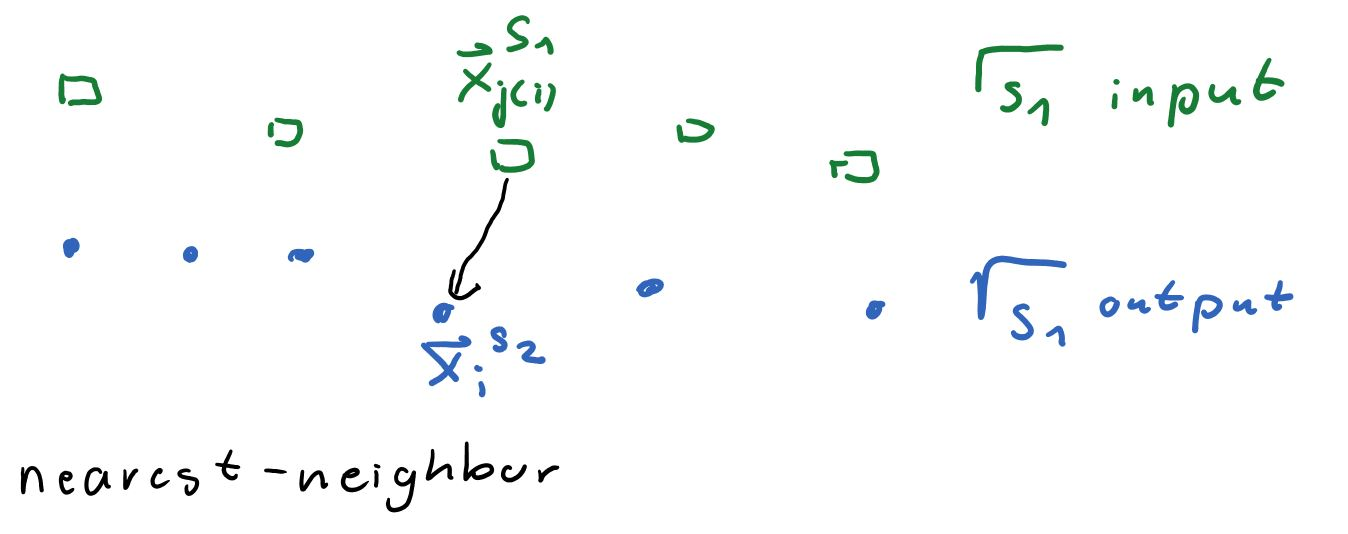
\includegraphics[width=0.95\textwidth]{figs/nn_points.jpg}
    \begin{tikzpicture}[x=15mm, y=15mm]
      \foreach \x in {0,1,...,4} {
        \node[inNode] (in\x) at (\x/2, 0) {};
      }
      \foreach \x in {0,1,...,5} {
        \node[outNode] (out\x) at (\x/2.5, -0.4) {};
      }
      \node[anchor=south west] at (1,  0.1) {\textcolor{incolor}{$\mathcal{M}_{S_1}$ input}};
      \node[anchor=north west] at (1, -0.5) {\textcolor{outcolor}{$\mathcal{M}_{S_2}$ output}};

      \node[anchor=south] at (in0)  {$\vec{x}_j^{S_1}$};
      \node[anchor=north] at (out0)  {$\vec{x}_i^{S_2}$};

      \draw[-latex] (in0) -- (out0);
      \draw[-latex] (in1) -- (out1);
      \draw[-latex] (in2) -- (out2);
      \draw[-latex] (in2) -- (out3);
      \draw[-latex] (in3) -- (out4);
      \draw[-latex] (in4) -- (out5);
    \end{tikzpicture}
  }
  \subcaptionbox{}{%
    %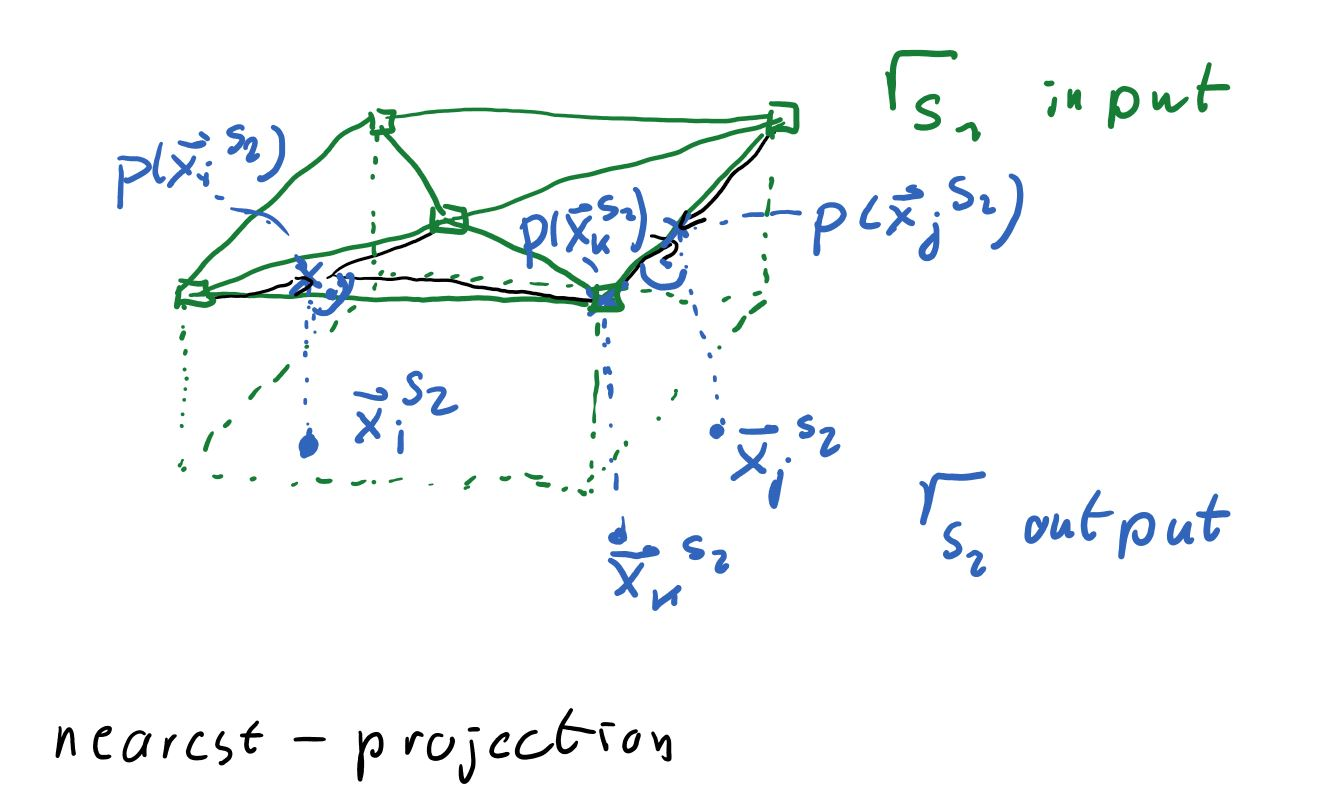
\includegraphics[width=0.95\textwidth]{figs/np_points.jpg}
    \begin{tikzpicture}[x=15mm, y=15mm]
      % bottom frame first
      \draw[dashed,incolor] (0, -1, 0) -- (2, -1, 0) -- (2, -1, 2) -- (0, -1, 2) -- cycle;
      \foreach \x in {0, 2} \foreach \y in {0, 2} {
        \draw[dashed,incolor] (\x, -0, \y) -- (\x, -1, \y);
      }

      % top nodes
      \node[inNode] (in0) at (0, 0, 0) {};
      \node[inNode] (in1) at (2, 0, 0) {};
      \node[inNode] (in2) at (2, 0, 2) {};
      \node[inNode] (in3) at (0, 0, 2) {};

      % top node connectivity
      \draw[thick, incolor] (in0) -- (in1) -- (in2) -- (in3) -- (in0) (in1) -- (in3);

      \node[anchor=south west] at (2,0,0) {\textcolor{incolor}{$\mathcal{M}_{S_1}$ input}};
      \node[anchor=north west] at (2,-1,2) {\textcolor{outcolor}{$\mathcal{M}_{S_2}$ output}};

      % triangle projection
      \path (0.5, 0, 0.7) 
        node[projNode] (tp) {} 
        node[above right] {$p(\vec{x}_1^{S_2})$}
        +(0,-1,0)
        node[outNode] (to) {} 
        node[right] {$\vec{x}_1^{S_2}$};
      \draw[-latex] (tp) -- (to);
      \draw pic [draw, angle radius=5pt, angle eccentricity=.5,pic text=.] { right angle = in3--tp--to };
      \draw[thin, dotted] (in0) -- (tp);
      \draw[thin, dotted] (in1) -- (tp);
      \draw[thin, dotted] (in3) -- (tp);

      % edge projection
      \path (2, 0, 1) 
        node[projNode] (ep) {} 
        node[right] {$p(\vec{x}_2^{S_2})$}
        -- +(0.2,-1,0)
        node[outNode] (eo) {} 
        node[right] {$\vec{x}_2^{S_2}$} ;
      \draw[-latex] (ep) -- (eo);
      \draw pic [draw, angle radius=5pt, angle eccentricity=.5,pic text=.] { right angle = in2--ep--eo };

      % node "projection"
      \path (0, 0, 2) 
        node[projNode] (vp) {} 
        node[left] {$p(\vec{x}_3^{S_2})$}
        -- +(-0.1,-1,0.5)
        node[outNode] (vo) {} 
        node[left] {$\vec{x}_3^{S_2}$};
      \draw[-latex] (vp) -- (vo);
    \end{tikzpicture}
  }
  \caption{\label{fig:nn_np}Basic principles of nearest-neighbor and nearest-projection mapping: (a) Transfer of each value $v_{j(i)}^{S_1}$ at the nearest neighbor $\vec{x}_{j(i)}^{S_1}$ in the coupling mesh of $S_1$ to the vertex $\vec{x}_i^{S_2}$ in the coupling mesh of $S_2$. (b) Projection of points $\vec{x}_1^{S_2}$, $\vec{x}_2^{S_2}$, and $\vec{x}_3^{S_2}$ of the coupling mesh of $S_2$ to a triangle, an edge, and a vertex, respectively, of the coupling mesh of $S_1$.}
\end{figure}  

Both nearest-neighbor and nearest-projection mapping require neighbor search between mesh entities of both participants. 
To implement this search efficiently, we generate r-start index-trees for vertices, edges, and triangles of meshes using the Geometry package of Boost\footnote{Boost C++ libraries: \url{https://boost.org/}.}.
The complexity of generating the index tree is $O(n \log(n))$ and the complexity of each nearest neighbor query is $O(\log(n))$ if $n$ is the number of entities in the involved meshes. 

\subsubsection{Data mapping with radial basis functions}

Radial basis function (RBF) mapping uses a linear combination of radially symmetric basis functions centered at vertices $\vec{x}^{S_1}_{i}$ of the input mesh to create a global interpolation function, which is afterwards sampled at the vertices of the output mesh $\vec{x}^{S_1}_{i}$. In order to ensure that constant and linear functions are interpolated exactly, an additional global first-order polynomial term $q(\vec{x})$ is added to the interpolant $s : \mathbb{R}^{d} \rightarrow \mathbb{R}$:

\begin{equation*}
s \left( \vec{x} \right) = \sum\limits_{i=1}^{n_1} \lambda_{i} \cdot \phi \left( \| \vec{x} - \vec{x}^{S_1}_{i} \| _{2}\right) + q \left( \vec{x} \right) ,
\end{equation*}

where the radial basis function is given by $\phi$, and the polynomial term $q \left( \vec{x} \right) = \beta_{0} + \beta_{1} x_{1} + \ldots + \beta_{d} x_{d}$.
Several basis functions available in preCICE are listed in \autoref{BasisFunc}.
See \autoref{fig:rbf} for a schematic view of the relation between the vertices of both coupling meshes and the construction and evaluation of the interpolant.

\begin{table}[h!]
\centering
\caption{Radial basis functions available in preCICE (excerpt). Local basis functions have a support radius $r$, i.e., $\phi \left(\Vert \vec{x} \Vert_{2}\right) = 0$ for $\Vert \vec{x} \Vert_{2} > r$. C-TPS use normalized variables $\xi = \Vert \vec{x} \Vert_{2}/r$ and are set to zero for $\xi>1$. We enforce a finite support radius for Gaussians by setting the basis function to zero when falling below a threshold of $10^{-9}$~\cite{Lindner2017}. For a given support $r$, we can, thus, compute the necessary shape parameter $\zeta$.}
\label{BasisFunc}
\begin{tabular}{lcl}\toprule
& Basis Function & Support \\ \midrule
Gaussians    & $\exp^{-(\zeta \cdot \Vert \vec{x} \Vert)^{2}}$  & Local  \\
%Multiquadratics & $\sqrt{\zeta^{2} + \Vert \vec{x} \Vert ^{2}}$  & Global  \\
Global Thin Plate Splines (G-TPS) & $\Vert \vec{x} \Vert ^{2} \log(\Vert \vec{x} \Vert)$ & Global \\
%Compact Polynomial C0   & $(1 - \xi)^{2}$   & Local  \\
Compact Thin Plate Splines C2 (C-TPS)  & $1 - 30\xi ^{2} - 10\xi ^{3} + 45\xi ^{4} - 6\xi ^{5} - 60\xi ^{3}\log\xi$   & Local  \\
%Compact Polynomial C6  & $(1 - \zeta)^{8}(32\xi ^{3} + 25\xi ^{2} + 8\xi + 1)$   & Local   \\
\bottomrule
\end{tabular}
\end{table}

\begin{figure}[h!]
  \centering
  %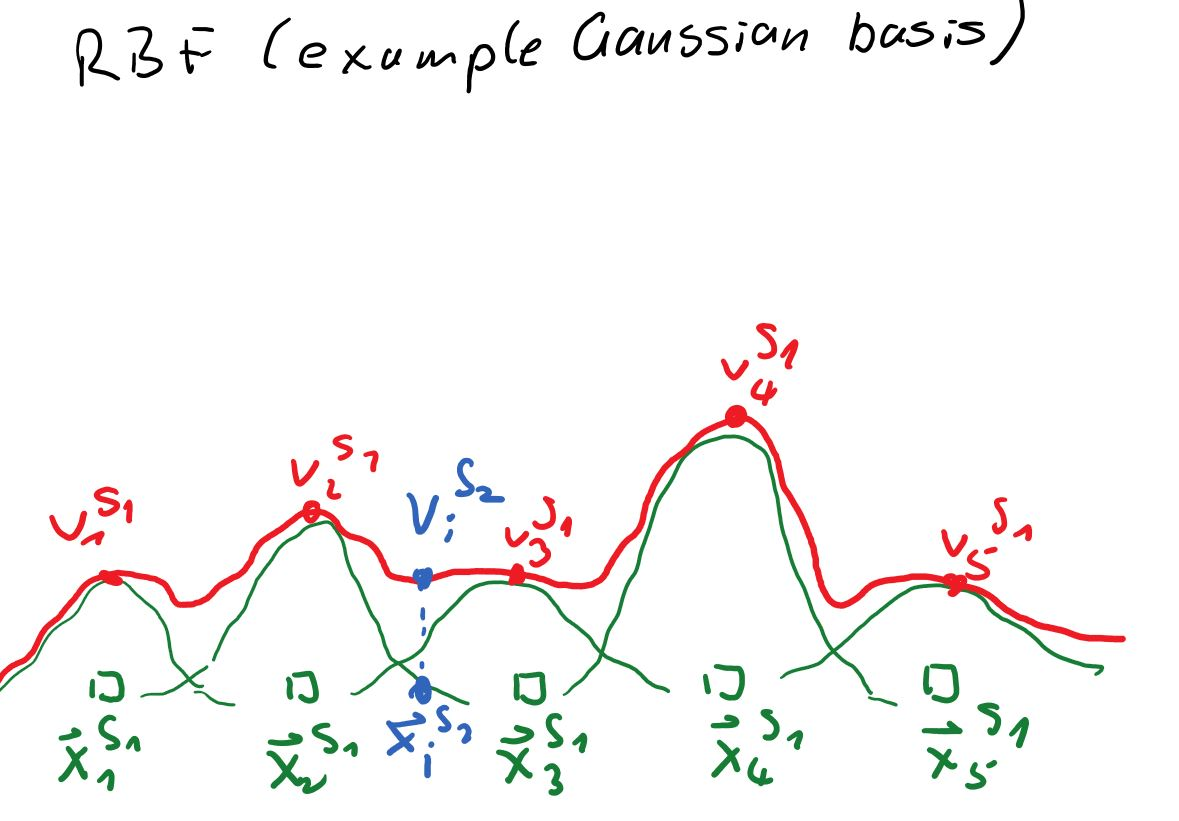
\includegraphics[width=0.95\textwidth]{figs/rbf_mapping.jpg}
  \begin{tikzpicture}[x=15mm, y=15mm]
    % Individual gaussians
    \draw[gray, shift={(1, 0)}, domain=-0.8:1.8,samples=200] plot(\x,{0.8*exp(-pow(\x/0.6, 2)/2)/(0.6*sqrt(2*pi))});
    \draw[gray, shift={(2, 0)}, domain=-1.8:1.8,samples=200] plot(\x,{1.2*exp(-pow(\x/0.6, 2)/2)/(0.6*sqrt(2*pi))});
    \draw[gray, thick, shift={(3, 0)}, domain=-1.8:1.8,samples=200] plot(\x,{0.9*exp(-pow(\x/0.6, 2)/2)/(0.6*sqrt(2*pi))});
    \draw[gray, shift={(4, 0)}, domain=-1.8:1.8,samples=200] plot(\x,{1.5*exp(-pow(\x/0.6, 2)/2)/(0.6*sqrt(2*pi))});
    \draw[gray, shift={(5, 0)}, domain=-1.8:0.8,samples=200] plot(\x,{0.7*exp(-pow(\x/0.6, 2)/2)/(0.6*sqrt(2*pi))});

    % support radius of middle gaussian
    \coordinate (mgl) at (1.2,0);
    \coordinate (mgr) at (4.8,0);
    \coordinate (sr) at (0,-0.5);

    \draw[gray, thin] (mgl) +(0,3pt) -- (mgl|-sr) -- +(0,-3pt);
    \draw[gray, thin] (mgr) +(0,3pt) -- (mgr|-sr) -- +(0,-3pt);
    \draw[gray, thin, latex-latex] (mgl|-sr) -- node[black,midway, below] {$2r$} (mgr|-sr);

    %\draw[gray, thin] (4.8, 0) +(0,2pt) -- (sr);
    %\draw[gray, thin] (4.8, 0) +(0,2pt) -- (sr);


    % Sum of all gaussians
    \draw[thick, name path=in, shift={(0, 0)}, domain=0.2:5.8,samples=200] plot(\x,{%
        0.8*exp(-pow((\x-1)/0.6, 2)/2)/(0.6*sqrt(2*pi)) +
        1.2*exp(-pow((\x-2)/0.6, 2)/2)/(0.6*sqrt(2*pi)) +
        0.9*exp(-pow((\x-3)/0.6, 2)/2)/(0.6*sqrt(2*pi)) +
        1.5*exp(-pow((\x-4)/0.6, 2)/2)/(0.6*sqrt(2*pi)) +
        0.7*exp(-pow((\x-5)/0.6, 2)/2)/(0.6*sqrt(2*pi))});

    % The bottom points and their top projection onto the sum of gussians
    \foreach \i in {1,2,3,4,5} {
      \node[inNode] (in\i) at (\i, 0) {};
      \node[anchor=north] at (in\i) {$\vec{x}_\i^{S_1}$};

      \path[name path=h\i] (\i,0) -- (\i,2);
      \path[name intersections={of=in and h\i, by=p\i}];
      \node[inNode] at (p\i) {};
      \node[anchor=south] at (p\i) {$v_\i^{S_1}$};
      \draw[dashed, incolor] (in\i) -- (p\i);
    }

    \node[outNode] (inI) at (2.5, 0) {};
    \node[anchor=north] at (inI) {$\vec{x}_i^{S_2}$};

    \path[name path=hI] (inI) -- +(0,2);
    \path[name intersections={of=in and hI, by=pI}];

    \node[projNode] at (pI) {};
    \draw[densely dashed] (inI) -- (pI);
    \node[anchor=south] at (pI) {$v_i^{S_2}$};
  \end{tikzpicture}
  \caption{\label{fig:rbf}Simplified one-dimensional view of the generation of the interpolant and the evaluation at the target point $\vec{x}_i^{S_2}$ based on a linear combination of Gaussian basis functions with support radius $r$, neglecting the global polynomial.}
\end{figure}  


The set of coefficients $\lambda_{i} \in \mathbb{R}, i=1,...,n_{S_1}$ is determined such that the interpolation conditions
%
\[
s \left( \vec{x}_{i}^{S_1} \right) = v_{i}^{S_1} \quad \forall i = 1,...,n_1 
\]
%
are fulfilled. The addition of the polynomial term leads to an under-determined system which is regularized by the polynomial conditions
%
\[
\sum\limits_{i=1}^{n_{S_1}} \lambda_{i} \cdot \vec{x}_{i}^{S_1} = 0 \; \mbox{ and } \; \sum\limits_{i=1}^{n_{S_1}} \lambda_{i} = 0.
\]
In matrix notation, this leads to the linear system
%
\[ \left( \begin{array}{cc} C & Q \\ Q^T & \mathbf{0} \end{array} \right) 
   \left( \begin{array}{c} \vec{\lambda} \\ \vec{\beta} \end{array} \right) = 
   \left( \begin{array}{c} \vec{v}^{S_1} \\ \vec{0} \end{array} \right), \]
% 
where $\vec{\lambda} = \left( \lambda_1, \lambda_2, \ldots, \lambda_{n_1} \right)^T$, $\beta = \left(\beta_0, \beta_1, \ldots, \beta_d\right)^T$, $C = \left( \phi \left( \Vert \vec{x}_{i}^{S_1} - \vec{x}_{j}^{S_1} \Vert_{2} \right) \right)_{i,j = 1, \ldots, n_1} \in \mathbb{R}^{n_1 \times n_1}$, $Q = \left( 1,\ x_{1,i}^{S_1},\ \ldots,\ x_{d,i}^{S_1} \right)_{i=1,\ldots,n_1} \in \mathbb{R}^{n_1 \times (d+1)}$
%
and, finally, the mapping reads
\[ \vec{v}^{S_2}  = \left( \begin{array}{cc} \tilde{C} & \tilde{Q} \end{array} \right) \left( \begin{array}{cc} C & Q \\ Q^T & \mathbf{0} \end{array} \right)^{-1} \left( \begin{array}{c} \vec{v}^{S_1} \\ \vec{0} \end{array} \right) \] 
with $\tilde{C} = \left( \phi \left( \Vert \vec{x}_{i}^{S_2} - \vec{x}_{j}^{S_1} \Vert_{2} \right)\right)_{\substack{i=1,\ldots, n_2 \\ j=1,\ldots,n_1}} \in \mathbb{R}^{n_2 \times n_1}$, 
$\tilde{Q} = \left( 1,\ x_{1,i}^{S_2},\ x_{2,i}^{S_2},\ x_{3,i}^{S_2} \right)_{i=1,\ldots,n_2} \in \mathbb{R}^{n_2 \times 4}$.

Local basis functions result in a sparse matrix $C$. 
However, the polynomial term matrix $Q$ is always densely populated, which hampers the favorable properties of the sparse matrix. Solving the polynomial term separately in a least squares approach via QR-decomposition of the matrix $Q$ capitalizes on the sparsity of the matrix $C$. For a full description of this separated polynomial approach, the reader is referred to~\cite{Lindner2017}.


As radial basis functions are radially symmetric in all spatial dimensions, distances between the two involved coupling meshes normal to a coupling surface do not have to be explicitly tackled, in contrast to the nearest-projection method. However, the accuracy of the RBF mapping decreases with an increasing gap or overlap between the two meshes of $S_1$ and $S_2$. In addition, the RBF mapping with local basis functions suffers from a trade-off between high accuracy (achieved for basis functions with wide support) and feasible conditioning of the linear system (only given for moderate support width). We address the latter to some extent by scaling the interpolant with the interpolant of the constant unit function, which allows us to use a smaller support radius without deteriorating accuracy~\cite{deparis2014rescaled, Lindner2017}.

%\[
%s_{r} = \frac{s \left( \vec{x} \right)}{s_{1} \left( \vec{x} \right)} ,
%\]
%where $s_{1} \left( x \right)$ is the interpolant constructed for the constant function $g \left( \vec{x} \right) = 1$.  

The RBF data mapping is implemented using either (depending on configuration) an iterative GMRES solver from PETSc~\cite{petsc-user-ref} in every mapping step, or an initial dense QR-decomposition from Eigen~\cite{eigenweb} followed by a matrix-vector product and a backward substitution in every mapping step. While the GMRES solver is fully parallelized, the QR-decomposition uses a sequential computation on a single rank.


\subsubsection{Numerical and performance results}

We compare the various data mapping methods in terms of accuracy and computational demand using the Abstract Solver Testing Environment (ASTE)\footnote{ASTE branch used for these tests: \url{https://github.com/precice/aste/tree/mapping-tests}}. ASTE imitates data input and output of participants coupled via preCICE in an artificial setting. In our test setup, two ASTE participants, $S_1$ and $S_2$, are coupled via preCICE. Both define individual surface meshes of the same geometry. We then use an analytical test function,
\[
  f(\vec{x}) = 0.78 \cdot \cos \left(10 \cdot (x_1 + x_2 + x_3)\right)\;,
\]
to set values on $\mathcal{M}_{S_1}$. We compute a single consistent mapping from $\mathcal{M}_{S_1}$ to $\mathcal{M}_{S_2}$ and measure errors on $\mathcal{M}_{S_2}$ with a discrete $l_2$-norm,
\[
\frac{1}{n} \left(\sum_{i=1}^n \left(v_i^{S_1} - f(\vec{x}^{S_1}_i)\right)^2 \right)^{\frac{1}{2}}\;.    
\]
The mapping error procedure is shown in Algorithm~\ref{alg:mapError}.

\begin{algorithm}[H]
  \caption{Data mapping error procedure}
  \label{alg:mapError}
  \begin{algorithmic}[1]
    \State Fix the output mesh $S_2$ while varying the input mesh $S_1$
    \State Apply test function on mesh $S_1$: $v^{S_1}_{i,real} = f(x^{S_1}_i)$ and B: $v^{S_2}_{i,real} = f(x^{S_2}_i)$
    \State Run mapping from $S_1$ to $S_2$ with $v^{S_1}_{i,real}$, resulting in data $v^{S_2}_{i,interpolant}$
    \State Compute per vertex error  $e_i = | v^{S_2}_{i,interpolant} - v^{S_2}_{i,real} |$
    \State Compute relative-l2 error $e' = \frac{1}{n} \left(\sum_{i=1}^n e_{i}^2 \right)^{\frac{1}{2}}\;.$
  \end{algorithmic}
\end{algorithm}

As test geometry, we use a turbine blade\footnote{Wind Turbine Blade created by Ivan Zerpa \url{https://grabcad.com/library/wind-turbine-blade--4}}. We use GMSH\cite{geuzaine2009gmsh} to generate almost uniform surface meshes with different resolutions as listed in \autoref{tab:meshes}. In \autoref{fig:geometry}, we visualize the geometry, different meshes, and the test function. 

\begin{table}[h!]
  \centering
  \caption{The meshes used for the mapping tests sorted from fine to coarse. Bold typesetting indicates the output meshes (associated to participant $S_2$). All other meshes are used as input meshes (associated to participant $S_1$).}
  \label{tab:meshes}
  \begin{tabular}{lrrc}
    \toprule
    $h$    & Vertices & Triangles & Series          \\
    \midrule
    0.03   & 438      & 1007      & coarse          \\
    0.02   & 924      & 2027      & coarse          \\
    0.01   & 3458     & 7246      & coarse          \\
    0.009  & 4302     & 8970      & \textbf{coarse} \\
    0.008  & 5310     & 11025     & coarse          \\
    0.006  & 9588     & 19712     & coarse          \\
    0.004  & 21283    & 43352     & fine, coarse    \\
    0.003  & 38112    & 77271     & fine            \\
    0.002  & 84882    & 171319    & fine            \\
    0.0014 & 172803   & 347815    & \textbf{fine}   \\
    0.001  & 338992   & 681069    & fine            \\
    0.0007 & 691426   & 1387249   & fine            \\
    0.0005 & 1354274  & 2714699   & fine            \\
    \bottomrule
  \end{tabular}
\end{table}

\begin{figure}[h!]
  \centering
  \begin{tikzpicture}[x=.2\textwidth]
    \node at (0,0) {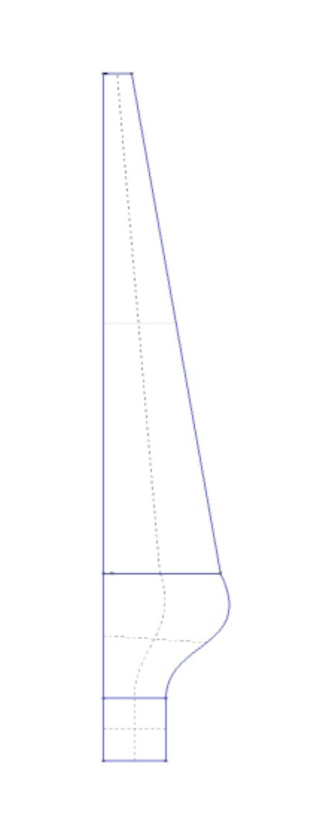
\includegraphics[width=.2\textwidth,keepaspectratio]{figs/mapping/mesh/turbine-geo.jpg}};
    \node at (1,0) {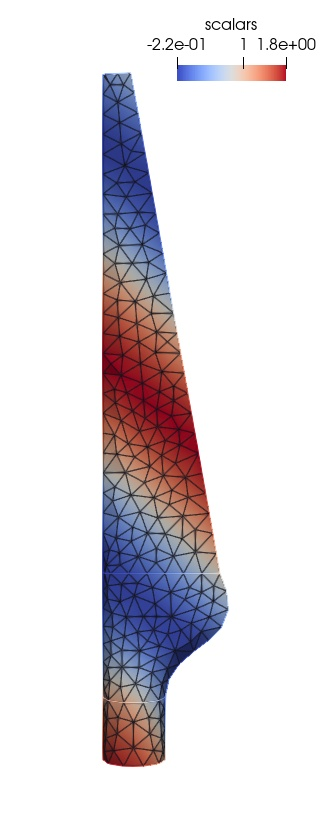
\includegraphics[width=.2\textwidth,keepaspectratio]{figs/mapping/mesh/turbine-0.03.jpeg}};
    \node at (2,0) {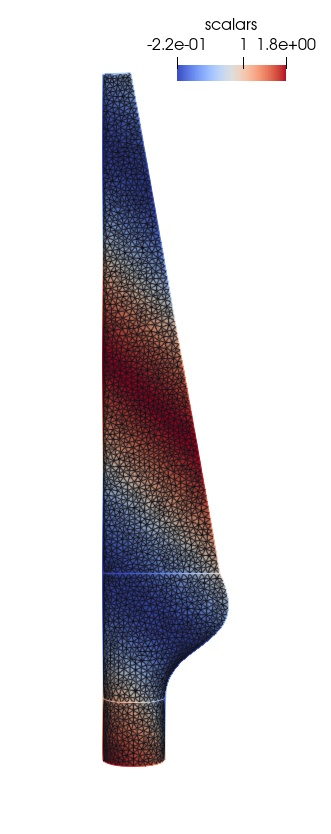
\includegraphics[width=.2\textwidth,keepaspectratio]{figs/mapping/mesh/turbine-0.009.jpeg}};
    \node at (3,0) {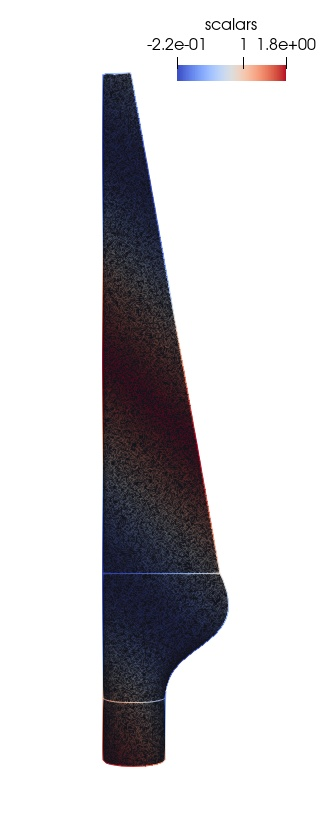
\includegraphics[width=.2\textwidth,keepaspectratio]{figs/mapping/mesh/turbine-0.004.jpeg}};
    \node at (4,0) {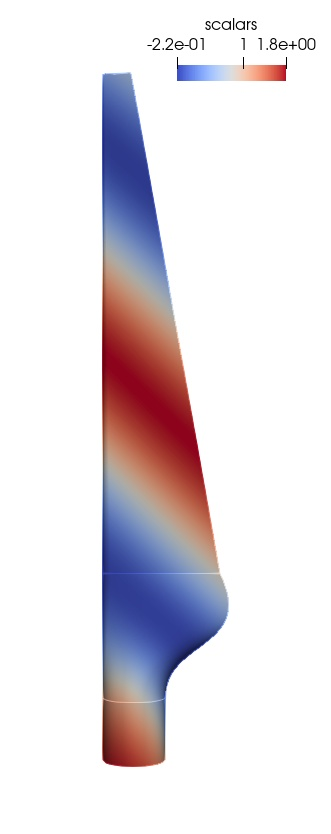
\includegraphics[width=.2\textwidth,keepaspectratio]{figs/mapping/mesh/turbine-0.0005.jpeg}};
  \end{tikzpicture}
  \caption{Mapping test case: Different meshes of the turbine-blade test geometry.
    From left to right: the geometry used to generate the meshes, $h=0.03$, $h=0.009$, $h=0.004$, $h=0.0005$ without edges.
    The mesh surface color indicated the test function, edges are drawn in black.
  }
  \label{fig:geometry}
\end{figure}

\begin{figure}[h!]
  \centering
  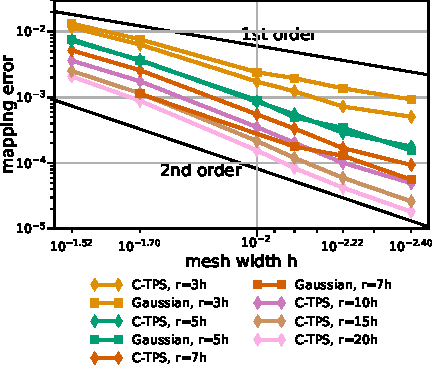
\includegraphics{figs/mapping/turbine-small-error-localrbf.pdf}
  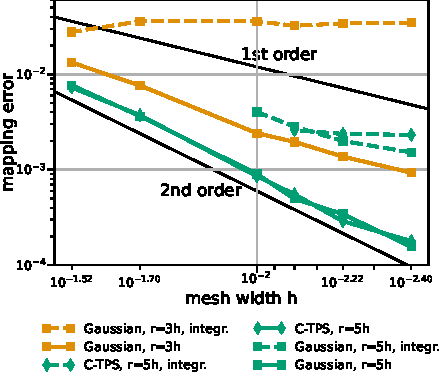
\includegraphics{figs/mapping/turbine-small-error-poly.pdf}
  \caption{%
    RBF data mapping with local basis functions for coarse series. Comparison of various support radii (left) and integrated and separated handling of the global polynomial (right).  
    Participant $S_2$ uses $h=0.009$. Missing data points mark diverging cases.
    Gaussians with $r=7h$ or $r=10h$ diverge for some or all cases, respectively (left).
    With integrated handling of the polynomial, both basis functions diverge for $r=5h$ and coarser meshes (right).}
  \label{fig:mapping_rbf_small}
\end{figure}

We run the mapping tests on the thin-nodes partition of SuperMUC-NG, hosted at the Leibniz Supercomputing Centre.  Each thin-node contains two 3.1GHz Intel Xeon Platinum 8174 (SkyLake) processors with a total of 48 cores and 96GB of system memory per node.  The tests used the Intel Omni-Path interconnect as primary network connection.
We run participant $S_1$ on a single node (48 MPI ranks) and participant $S_2$ on two nodes (96 MPI ranks) as participant $S_2$ computes the actual mapping. Runtime is the maximum of a given event over all ranks of $S_2$\footnote{preCICE measures timings for a wide range of events across MPI ranks using the \github{precice/EventTimings} framework.} and memory is the sum of the peak memory usage of all ranks of $S_2$. These results are in addition averaged over five runs.
For the RBF data mapping variants, we use GMRES as linear solver with a relative convergence threshold of $10^{-6}$, except for G-TPS, where we use the sequential QR-decomposition.

We compare the data mapping methods in two series of computations. The first, \textit{coarse} series is based on meshes with $h \geq 0.004$, where participant $S_2$ always uses $h=0.009$ and participant $S_1$ varies the value of $h$ through all other values of the series listed in \autoref{tab:meshes}. The second, \textit{fine} series is based on meshes with $h \leq 0.004$. Participant $S_2$ uses $h=0.00014$ and participant $S_1$ the rest. While we can compare all mapping variants for the coarse series, RBF data mapping with G-TPS is too expensive in terms of computation and memory for the fine series.
For reproduction of our results, all data used as well as all steps are available in an archive\footnote{Test Setup: \url{https://gitlab.lrz.de/precice/precice2-ref-paper-setup}}.

\autoref{fig:mapping_rbf_small} gives results for RBF data mapping with local basis functions -- C-TPS and Gaussians -- for varying support radii and for integrated and separated handling of the global polynomial.
Separated handling of the polynomial clearly outperforms integrated handling in terms of accuracy and robustness. For C-TPS, an increase in accuracy is observed for increasing support radius. This is even true for rather large radii ($r=20h$), where we get more than quadratic convergence. Gaussians, however, show robustness issues for larger support radii. We assume that this behavior is caused by the increasing ratio of large to small matrix entries. In a further test (not shown here), we observed that increasing the (hard-coded) threshold value from $10^{-9}$ to $10^{-5}$ seems to improve robustness.

\autoref{fig:mapping_all_small} sets the best local RBF variants in perspective with RBF mapping using G-TPS, nearest-neighbor mapping, and nearest-project mapping. 
RBF mapping using C-TPS with a large support radius is comparable to RBF mapping using G-TPS. The latter only wins for the finest meshes. RBF data mappings clearly outperform nearest-neighbor and nearest-projection mapping -- even for a relatively small support radius of $h=3r$. Nearest-projection mapping, interestingly, does not show a constant second-order convergence for the coarse series, which suggests that the projection error dominates the interpolation error. In fact, similar tests with a cubic geometry (not shown) give constant second-order convergence for nearest-projection mapping as, in this case, all meshes directly lie on the geometry (i.e.~no projection error). For the fine series, nearest-projection mapping gives a rather constant second-order convergence as well. 


\begin{figure}[h!]
  \centering
  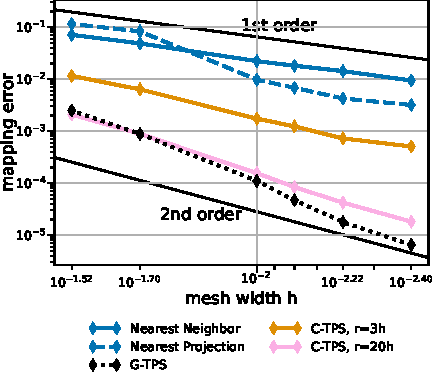
\includegraphics{figs/mapping/turbine-small-error-best.pdf}
  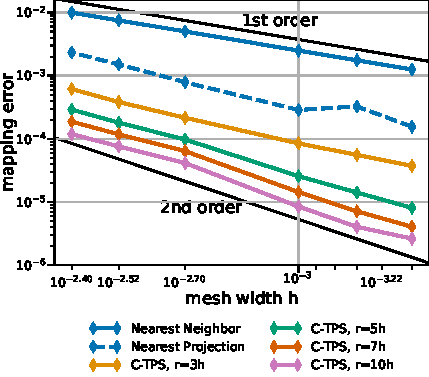
\includegraphics{figs/mapping/turbine-big-error-best.pdf}
  \caption{%
    Comparison of nearest-neighbor / nearest-projection mapping and RBF mapping with G-TPS and C-TPS for coarse series (left) and fine series (right) from \autoref{tab:meshes}. RBF mapping with G-TPS is infeasibly expensive for the fine series. All RBF mapping methods use a separated handling of the polynomial.
    Participant $S_2$ uses $h=0.009$ for the coarse series (left) and $h=0.0014$ for the fine series (right).
  }
  \label{fig:mapping_all_small}
\end{figure}

Next, we compare the same methods in terms of compute time. Here, we have to distinguish between one-time preparation time (e.g., QR-factorization, matrix initialization in PETSc, or nearest-neighbor search) and recurrent mapping time in every mapping operation (e.g., back substitution or GMRES solve). \autoref{fig:mapping_time_coarse} and \autoref{fig:mapping_time_fine} give both data for various data mapping methods and the coarse and fine series, respectively. The quickly increasing preparation time of RBF mapping with G-TPS makes the method unpractical for finer meshes. For C-TPS, both the preparation time and the recurrent mapping time increases significantly with increasing support radius and decreasing mesh width. For fine meshes, larger support radii are thus discouraged despite their superior accuracy. For small cases, the overhead of the PETSc solver for RBF is more costly than the overall serial QR-factorization in G-TPS. Nearest-neighbor and nearest-projection mapping are both drastically cheaper than RBF data mapping, particularly in the recurrent mapping time. Finally, \autoref{fig:mapping_memory} compares the peak memory consumption of all data mappings. RBF mapping with G-TPS shows a drastic increase in memory with increasing mesh size. For the coarse series, all methods show the expected behavior: higher memory consumption for RBF than for nearest-neighbor and nearest-projection mapping and increasing memory consumption for RBF mapping using C-TPS with increasing support radius.
For the fine series, the nearest-project surpassed even the RBF methods, due to the additional cost of handling connectivity information.


\begin{figure}[h!]
  \centering
  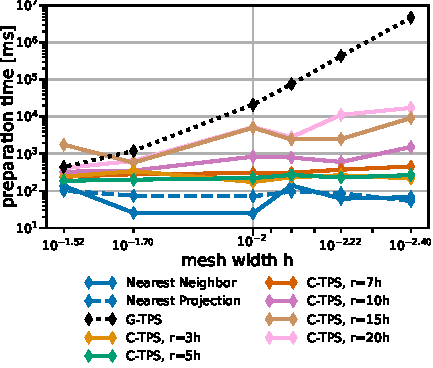
\includegraphics{figs/mapping/turbine-small-computet.pdf}
  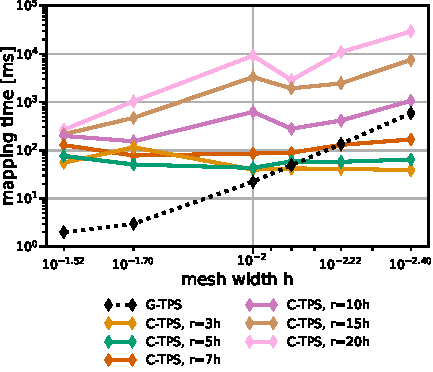
\includegraphics{figs/mapping/turbine-small-mapt.pdf}
  \caption{%
    Comparison of one-time preparation time (left) and the recurrent mapping time (right) of various data mapping methods for the coarse series from \autoref{tab:meshes}. All RBF mapping methods use a separated handling of the polynomial.
    The recurrent mapping time of nearest-projection and nearest-neighbor mapping is below the measurement resolution of $1ms$ and hence omitted.
    Participant $S_2$ uses $h=0.009$.
  }
  \label{fig:mapping_time_coarse}
\end{figure}

\begin{figure}[h!]
  \centering
  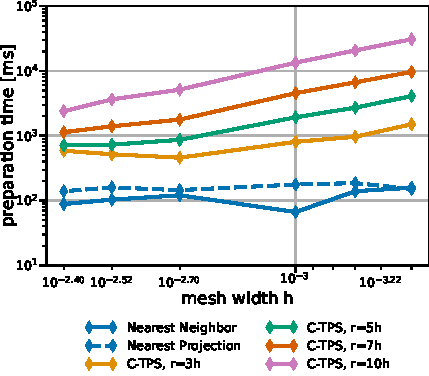
\includegraphics{figs/mapping/turbine-big-computet.pdf}
  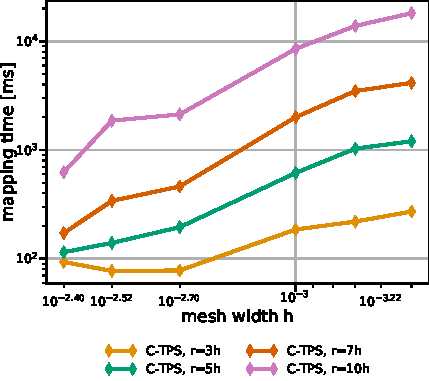
\includegraphics{figs/mapping/turbine-big-mapt.pdf}
  \caption{%
    Comparison of one-time preparation time (left) and the recurrent mapping time (right) of various data mapping methods for the fine series. All RBF mapping methods use a separated handling of the polynomial.
    The one-time preparation of the nearest-neighbor mapping is an inexpensive operation and has the tendency to fluctuate, 5 samples are not enough to fully smooth them out resulting in a spike at $0.001$.
    The recurrent mapping time of nearest-projection and nearest-neighbor mapping is below the measurement resolution of $1ms$ and hence omitted.
    Participant $S_2$ uses $h=0.0014$.
  }
  \label{fig:mapping_time_fine}
\end{figure}

\begin{figure}[h!]
  \centering
  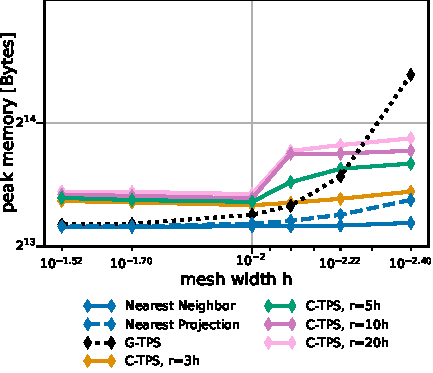
\includegraphics{figs/mapping/turbine-small-peakMemB.pdf}
  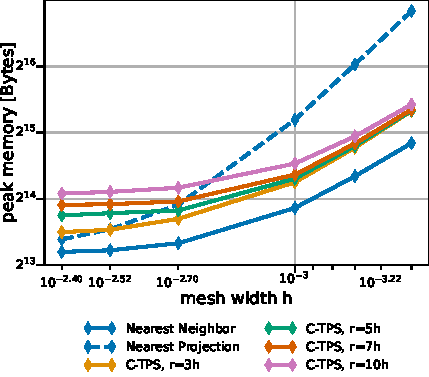
\includegraphics{figs/mapping/turbine-big-peakMemB.pdf}
  \caption{%
    Comparison of the maximum overall memory consumption of various data mapping methods for coarse series (left) and fine series (right) from \autoref{tab:meshes}.
    Participant $S_2$ uses $h=0.009$ for the coarse series (left) and $h=0.0014$ for the fine series (right).
    The memory consumption is the maximum of all ranks of participant $S_2$, which is executing the mapping.
  }
  \label{fig:mapping_memory}
\end{figure}

We conclude that RBF data mapping with local basis functions is a powerful method. There is a natural trade-off between accuracy and compute effort when modifying the support radius. A good compromise is a support radius of $r=5h$ to $r=7h$. In the current implementation, C-TPS should be preferred over Gaussians as basis functions. RBF mapping with G-TPS should only be used for small mesh sizes. 
When RBF data mapping becomes too expensive, nearest-projection mapping is a good alternative except for very large out-of-memory cases. 
Scalability results for the mapping computation were recently published in~\cite{AminPerf2021}. In addition, we aim for a more in-depth analysis of mapping variants with further geometries in future work. 


\subsection{Communication}
\label{ssec:com}

Besides coupling schemes and data mapping, the third feature pillar of preCICE is inter-code communication. For large-scale simulations on massively-parallel high-performance computing systems, efficient inter-code communication is a necessity. Employing any central instance not only deteriorates the communication performance, but can also be memory prohibitive when large amounts of data must be communicated. Therefore, preCICE implements fully parallel point-to-point communication~\cite{Uekermann2016, Bungartz2016_ExaFSA_LNCSE, Shukaev2015}. 
In the initialization phase, preCICE performs an analysis of the coupling mesh partitions and the defined data mappings of each connected pair of participants to find the list of required connections between the MPI ranks of either participant (cf.~\autoref{fig:comm}). 
To this end, bounding boxes around mesh partitions are compared in a first step, leading to preliminary communication channels. In a second step, actual mesh data is compared in a fully-parallel fashion~\cite{AminPerf2021}.

\begin{figure}[h!]
  \centering
  \begin{tikzpicture}
      \foreach \n in {0,1,2,3,4,5} {
        \node[inNode,inner sep=3pt] (a\n) at (0, \n) {};
      }
      \begin{scope}[every node/.style={outNode, inner sep=3pt}]
      \node (b0) at (2, 0.5) {};
      \node (b1) at (2, 1.5) {};
      \node (b2) at (2, 3.5) {};
      \node (b3) at (2, 4.5) {};
      \end{scope}

    \begin{scope}[line width=2pt]
      \foreach \n in {0,2,4} {
        \draw (a\n) ++(-0.5, -0.25) coordinate (au\n) -- ++(0,1.5) coordinate (ab\n);
      }
      \foreach \n in {0,2} {
        \draw (b\n) ++(0.5, -0.25) coordinate (bu\n) -- ++(0,1.5) coordinate (bb\n);
      }
    \end{scope}

    \path
      (a0) +(-0.5, 0.5) node[anchor=east] {$S_1^0$}
      (a2) +(-0.5, 0.5) node[anchor=east] {$S_1^1$}
      (a4) +(-0.5, 0.5) node[anchor=east] {$S_1^2$}
      (b0) +( 0.5, 0.5) node[anchor=west] {$S_2^0$}
      (b2) +( 0.5, 0.5) node[anchor=west] {$S_2^1$}
      ;

    \begin{pgfonlayer}{bg}
      \fill[gray!20] (au0) to[out=0,in=180,looseness=1.5] (bu0) -- (bb0) to[out=180,in=0] (ab0) -- cycle;
      \fill[gray!20] (au2) to[out=0,in=180] (bu0) -- (bb0) to[out=180,in=0] (ab2) -- cycle;
      \fill[gray!20] (au2) to[out=0,in=180] (bu2) -- (bb2) to[out=180,in=0] (ab2) -- cycle;
      \fill[gray!20] (au4) to[out=0,in=180] (bu2) -- (bb2) to[out=180,in=0,looseness=1.5] (ab4) -- cycle;
    \end{pgfonlayer}

    \draw[out=0,in=180,
      decoration={markings, mark=at position 0.5 with {\arrow[line width=1pt]{latex}}},
          every edge/.append style={postaction={decorate}},
      ] (a0) edge (b0) (a1) edge (b1) (a2) edge (b1) (a3) edge (b2) (a4) edge (b2) (a5) edge (b3) ;
  \end{tikzpicture}
  \caption{Communication initialization in preCICE.
    Given the distribution of vertices among the ranks of parallel participants $S_1^i$ and $S_2^j$,
    combined with a data mapping between the vertices shown in the middle,
    preCICE deduces the required communication pattern of ranks between participants $S_1$ and $S_2$, depicted as the gray connections.}
  \label{fig:comm}
\end{figure}

As communication backends, preCICE supports MPI and TCP/IP.
In general, communication via MPI is faster. However, TCP/IP communication is more robust and flexible, since not all MPI implementations support the necessary inter-code MPI functionality. For MPI-based communication, preCICE creates a single inter-code communicator including all involved ranks from both participants. To establish TCP/IP-based connections, on the other hand, each pair of connected ranks exchanges a connection token via the file system. To reduce the load on the file system, a hash-based scheme is used, which distributes the connection files uniformly across different directories~\cite{Lindner2020_ExaFSA, Lindner2019}. This minimizes the number of files per directory, and, thus, improves efficiency and increases the feasible number of connections.

\subsection{Getting and building preCICE}
\label{ssec:building}

After introducing the basic coupling methods implemented in preCICE in the last three sections, we now give an overview of various ways to get preCICE.
The GitHub repository\footnote{preCICE repository on GitHub: \url{www.github.com/precice/precice}} is the central platform for development,
issue tracking, and contributing. It provides the release timeline with release notes, automatic source archives, and build artifacts. However, the repository 
% Well integrated with other services (static analysis, code coverage, CI)
only contains the preCICE library and native (C and Fortran) language bindings. Additional derived software is hosted in separate repositories under the preCICE GitHub organization: 
adapter codes, tutorials, Python and MATLAB language bindings, and more.
All these components, together with the core library, are part of the \textit{preCICE distribution}\footnote{preCICE distribution: \url{https://precice.org/installation-distribution.html}}, a versioned and citable ecosystem of components that are meant to work together and are maintained by the preCICE developers. Everything presented in this paper refers to the version v2104.0 of the distribution~\cite{Chourdakis2021_Distribution}.

On the other hand, the preCICE library also depends on various other libraries for a range of features. See \autoref{table:dependencies} for an overview of dependencies and their associated features in preCICE.

\begin{table}[h!]
  \begin{tabular}{lllp{5cm}}\toprule
    Dependency       & Version & CMake Option                       & Features                                               \\\midrule
    Boost Geometry   & $\geq$ 1.65.1  & \textit{required}                  & Spacial index trees                                    \\
    Boost Container  & $\geq$ 1.65.1  & \textit{required}                  & Flat maps and sets                                     \\
    Boost Stacktrace & $\geq$ 1.65.1  & \textit{required}                  & Stacktrace information                                 \\
    Boost Log        & $\geq$ 1.65.1  & \textit{required}                  & Configurable logging                                   \\
    Boost Test       & $\geq$ 1.65.1  & \textit{required}                  & Base of testing framework                              \\
    Eigen            & 3       & \textit{required}                  & Mesh representation and radial basis function mapping. \\
    libxml           & 2       & \textit{required}                  & Parsing of XML config files.                    \\
    PETSc            & $\geq$ 3.6     & \incode{PRECICE_PETScMapping}     & Parallel RBF mapping.                \\
    Python           & $\geq$ 3.6     & \incode{PRECICE_PythonActions}    & User-defined actions                                   \\
    NumPy            & $\geq$ 1.18.1  & \incode{PRECICE_PythonActions}    & User-defined actions                                   \\
    MPI              & MPI-3   & \incode{PRECICE_MPICommunication} & MPI communication back-end                             \\
    \bottomrule
  \end{tabular}
  \caption{Dependencies of preCICE and associated features in preCICE.}
  \label{table:dependencies}
\end{table}

A decision graph for getting preCICE is shown in \autoref{fig:install-decision}. We describe the different options in the following.

\paragraph{Debian packages for preCICE on Ubuntu}
Due to the popularity of Ubuntu among preCICE users, we provide corresponding Debian packages.
We aim to support the latest two Ubuntu \textit{long term support} (LTS) releases, which is frequency-wise compatible with our
strategy to not release new major versions (breaking changes) more often than every two to three years.
The Debian packages contained in our GitHub releases allow one-click installation on supported platforms.
This avoids explicit dependency management by the user. The current Debian package is always generated for 
the latest Ubuntu release as well as the latest Ubuntu LTS.

\paragraph{Building preCICE using Spack}
In addition, we maintain a Spack~\cite{spack} package which allows to build the complete required software stack
from source code. 
This is essential to be able to test arbitrary combinations of dependency versions and different compilers.
We actively maintain a build recipe with common
configurations. Moreover, preCICE is a member of the Extreme-scale Scientific Development Kit (xSDK) \footnote{xSDK: \url{http://xsdk.info/}} since \incode{xsdk-0.5.0} (November 2019)\footnote{See \url{https://github.com/xsdk-project/xsdk-policy-compatibility/blob/master/precice-policy-compatibility.md} for more details on all policies fulfilled by preCICE.}, which promises
compatibility to other major scientific computing packages.
% The current version of the Spack package only supports Linux. % It actually works on macOS
%macOS support will be available in the near future. 


%\begin{minted}{text}
%$ spack install preCICE
%$ spack install preCICE@2.0.0^mpich
%\end{minted}

\paragraph{Building preCICE with CMake}
For other platforms, we provide an in-depth guide on how to build preCICE from source. Versioned code archives are available for every release.
For cross-platform build system configuration, preCICE leverages the industry standard CMake.
It allows users and developers to develop and build in their environment of choice.
The adoption of CMake simplifies package generation and the future adoption of Windows and macOS support.
%As it is build system agnostic, the user needs to provide one build system (e.g., GNU make or ninja).
% Contributors should install Clang-format v8 and GNU Parallel for code style formatting
macOS works out-of-the-box since preCICE v2.2. There are several ways to support Windows:
Since v1.x, there is community support via MinGW.
Windows users that rely on WSL (Windows Subsystem for Linux) can install preCICE there normally.
We are currently preparing native Windows support (MSVC compiler), in addition. 

\paragraph{preCICE tutorials virtual machine image}
Before running their first coupled simulation, a user needs to install not only the preCICE library, but also a minimum set of adapters and third-party solvers.
This can become even more complicated if the user does not already work on a platform compatible with all components.
To lower the entry barrier, we provide a virtual machine (VM) image with all components needed to run the preCICE tutorials.
We create\footnote{preCICE VM sources: \url{https://github.com/precice/vm}} and distribute\footnote{preCICE Vagrant box: \url{https://app.vagrantup.com/precice/precice-vm}\\documentation: \url{https://precice.org/installation-vm.html}}
this image as a Vagrant\footnote{Vagrant: \url{https://github.com/hashicorp/vagrant}} Box,
which is currently available for VirtualBox, but could easily be packaged for other providers as well.
We chose Vagrant instead of a provider-specific system, as Vagrant allows us to highly automate the box generation,
integrates with the host system automatically (SSH access, shared folders),
provides infrastructure to distribute the box, and works with various host platforms and virtualization providers.
We chose a VM instead of a container-based system, as virtual machines provide access to a full graphical environment by default
and many users in our community already have experience working with virtual machines, but not with containers.


\begin{figure}[h!]
  \centering
  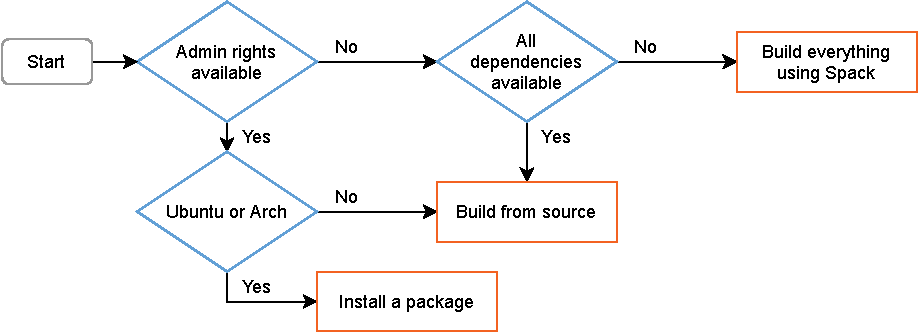
\includegraphics[width=\textwidth]{figs/installation/install-decision.pdf}
  \caption{Decision graph and overview of the different installation methods for preCICE on Linux.
  On macOS, users can build using Spack, or install dependencies from Homebrew and build from source.
  On Windows, preCICE is available from MINGW (experimental), while it can also work inside the Windows Subsystem for Linux.
  Before deciding to install preCICE on their system, users can try a
  virtual machine containing all the software needed to run the preCICE tutorials.}
  \label{fig:install-decision}
\end{figure}

\subsection{Application programming interface and configuration} 
\label{ssec:api}

Now that we know which coupling methods preCICE offers and how to get preCICE, we show in this section how preCICE can actually be used.
%
Even though preCICE is a C++ library, it also supports the  software programming languages most widely-used in simulation, as shown in \autoref{table:bindings}.
Alongside the native application programming interface (API) for C++, preCICE provides C and Fortran bindings by default.
The API for other languages is provided via independent projects, as they follow different release cycles, different project management, and different developer and installation procedures. Python bindings are based on Cython, installable via pip from PyPI. MATLAB bindings~\cite{Volland2019} are based on the MEX interface and Julia bindings are currently in the prototype phase. Finally, we develop an independent Fortran module for easier integration of preCICE into Fortran codes. The architecture and relation between these projects is described in the documentation\footnote{API documentation overview: \url{https://precice.org/couple-your-code-api.html}}. All language bindings also provide so-called \textit{solverdummies} as example codes and provide \incode{pkg-config} and \incode{CMakeConfig} files for integration into other projects.

\begin{table}[h!]
  \begin{tabular}{lll}\toprule
    Language       & Location                         & Installation                                   \\\midrule
    C++            & \github{precice/precice}         & \textit{native API}                            \\
    C              & \github{precice/precice}         & \inbash{cmake -DPRECICE_ENABLE_C=ON .}       \\
    Fortran        & \github{precice/precice}         & \inbash{cmake -DPRECICE_ENABLE_FORTRAN=ON .} \\
    Fortran Module & \github{precice/fortran-module}  & \inbash{make}                                  \\
    Python         & \github{precice/python-bindings} & \inbash{pip install pyprecice@2.0.2}           \\
    MATLAB         & \github{precice/matlab-bindings} & MATLAB script                                  \\
    Julia          & \github{precice/julia-bindings}  & Julia package (experimental)                   \\ 
    \bottomrule
  \end{tabular}
  \caption{Programming languages supported by preCICE. CMake options for C and Fortran bindings are set to ON by default.}
  \label{table:bindings}
\end{table}

To introduce the API of preCICE, we use an example: we develop an adapter for a fluid solver written in Python to couple it to an already adapted solid solver for fluid-structure interaction (FSI). Mathematically, we realize a Dirichlet-Neumann coupling: we use the kinematic interface condition as Dirichlet boundary condition in the fluid solver and the dynamic interface condition as Neumann boundary condition in the solid solver. 
Thus, concerning coupling data, we receive the deformation of the solid from the solid solver as displacement values at the coupling interface and we return forces on the coupling interface to the solid solver. 
This example problem is representative for many preCICE users: an existing (in-house) fluid solver should be coupled to an off-the-shelf solid solver, which is already adapted for preCICE. 
The simplified code of the uncoupled fluid solver is depicted in \autoref{code:original}. \incode{u} is the current solution, for example velocity and pressure values. We use an adaptive time step size, computed in line 3, and solve one time step in line 4.

\begin{listing}[h!]
\caption{Original uncoupled fluid solver in Python}
\small
\label{code:original}
\begin{minted}[mathescape,linenos,numbersep=5pt,gobble=0,frame=none,framesep=20mm,escapeinside=||,breaklines]{python}
u = initialize_solution()
while t < t_end: # main time loop
    dt = compute_adaptive_dt() 
    u = solve_time_step(dt, u) # returns new solution
    t = t + dt    
\end{minted}
\end{listing}


\paragraph{Creating a handle to preCICE} \autoref{code:example} shows the fully-coupled fluid solver. The preCICE API is used at multiple locations, which we explain in the following paragraphs. For the sake of simplicity, we do not develop a general stand-alone adapter, but directly use the preCICE API in the fluid code -- meaning, we develop an \textit{adapted code}. In \autoref{sec:adapters}, we give an overview of several \textit{real} adapters. As the fluid code is written in Python, we make use of the Python bindings of preCICE: preCICE is imported in line 1. In line 3, the solver interface of preCICE is created. We pass the name of the solver and the preCICE configuration file. The latter defines the overall coupling topology (who is coupled to whom) and the used coupling methods (acceleration, data mapping, communication, etc.). We come back to this file later. Moreover, for parallel coupled codes, we need to give the current parallel rank (here 0) and the number of ranks (here 1) to preCICE.
The solver interface is initialized in line 13. Here, preCICE performs several first steps, such as setting up internal data structures and creating communication channels. In the end, the solver interface is finalized in line 42. Internal data structures are torn down and communication channels are closed.


\paragraph{Coupling meshes} Coupling data and coupling meshes are referred to by IDs, which are collected in lines 5 to 8.
The coupling mesh is defined before the initialization in line 11. preCICE treats coupling meshes as (unstructured) clouds of vertices, arranged in two-dimensional arrays of size vertices by dimension. Certain features of preCICE (e.g., nearest-projection data mapping) require mesh connectivity in addition. To this end, edges, triangles, and quads can optionally be defined, a step which we do not show in the example. 
The control of the end of the simulation is handed over to preCICE in line 17 to steer a synchronized end of all participants.
On the coupling mesh, coupling data structures are accessed in lines 24 and 32. The example uses specific calls for the vector-valued displacement and force values. The displacement values are used as Dirichlet boundary condition, here depicted as additional input of \inpython{solve_time_step} in line 28. The force values are computed from the current solution by means of a helper function in line 31. 


\begin{listing}[h!]
\caption{An adapted fluid solver written in Python. While preCICE is a C++ library, bindings for C++, C, Fortran, Python, and MATLAB make it possible to couple a large variety of participants in a minimally invasive way.}
\small
\label{code:example}
\begin{minted}[mathescape,linenos,numbersep=5pt,gobble=0,frame=none,framesep=20mm,escapeinside=||,breaklines]{python}
import precice

|{\color{my_orange}interface}| = precice.Interface("Fluid", "precice-config.xml", 0, 1)

mesh_id = interface.get_mesh_id("Fluid-Mesh")

displ_id = interface.get_data_id("Displacement", mesh_id)
force_id = interface.get_data_id("Force", mesh_id)

positions = ... #define interface mesh, 2D array with shape (n, dim)
vertex_ids = |{\color{my_orange}interface}|.set_mesh_vertices(mesh_id, positions)

precice_dt = |{\color{my_orange}interface}|.initialize()

u = initialize_solution()

while |{\color{my_orange}interface}|.is_coupling_ongoing(): # main time loop
        
    if |{\color{my_orange}interface}|.is_action_required(precice.action_write_iteration_checkpoint()):
        u_checkpoint = u
        interface.mark_action_fulfilled(precice.action_write_iteration_checkpoint())    

    # returns 2D array with shape (n, dim)
    displacements = |{\color{my_orange}interface}|.read_block_vector_data(displ_id, vertex_ids)

    dt = compute_adaptive_dt() 
    dt = min(precice_dt, dt)
    u = solve_time_step(dt, u, displacements) # returns new solution
    
    # returns 2D array with shape (n, dim)
    forces = compute_forces(u) 
    |{\color{my_orange}interface}|.write_block_vector_data(force_id, vertex_ids, forces)
    
    precice_dt = |{\color{my_orange}interface}|.advance(dt)

    if |{\color{my_orange}interface}|.is_action_required(precice.action_read_iteration_checkpoint()):
        u = u_checkpoint
        |{\color{my_orange}interface}|.mark_action_fulfilled(precice.action_read_iteration_checkpoint())
    else: # continue to next time step 
        t = t + dt    

|{\color{my_orange}interface}|.finalize()

\end{minted}
\end{listing}

\paragraph{Configuration} \autoref{code:config} gives an excerpt of a fitting preCICE configuration for our FSI example. The dimension of the scenario is specified in line 1 and can be either two or three. Two participants, \incode{Fluid} and \incode{Solid}, are configured. \incode{Fluid} uses the mesh from \incode{Solid} in line 13. This way, we can define data mappings between both meshes in lines 16 and 17. Here, we use RBF data mappings with compact thin-plate splines as basis functions. In line 22, we configure a TCP/IP sockets connection between both participants. Finally, in lines 24 to 31, a serial implicit coupling between both participants with an IQN-ILS acceleration is defined. \incode{Fluid} is the first participant, meaning that it starts each iteration. preCICE comes with a standalone Python tool called \textit{Config Visualizer}\footnote{preCICE config visualizer: \url{https://github.com/precice/config-visualizer}}, which helps understanding and debugging preCICE configuration files. The tool generates graphviz dot files\cite{Ellson03graphviz}, which can be, for example, converted to PDF. The generated PDF output is shown in \autoref{fig:config} for the example configuration.

\begin{listing}[h!]
\caption{Excerpt of a preCICE configuration file. Two participants \incode{Fluid} and \incode{Solid} are coupled.}
\small
\label{code:config}
\begin{minted}[mathescape,linenos,numbersep=5pt,gobble=0,frame=none,framesep=20mm,escapeinside=||,breaklines]{xml}
<solver-interface dimensions="3">   
  <data:vector name="Force"/>
  <data:vector name="Displacement"/> 
 
  <mesh name="Fluid-Mesh">
    <use-data name="Displacement"/>
    <use-data name="Force"/>
  </mesh>
  <mesh name="Solid-Mesh"> ... </mesh>

  <participant name="Fluid">
    <use-mesh name="Fluid-Mesh" provide="yes"/>
    <use-mesh name="Solid-Mesh" from="Solid"/>
    <write-data name="Force" mesh="Fluid-Mesh"/>
    <read-data name="Displacement" mesh="Fluid-Mesh"/>
    <mapping:rbf-compact-tps-c2 from="Fluid-Mesh" constraint="conservative" .../>
    <mapping:rbf-compact-tps-c2 from="Solid-Mesh" constraint="consistent" .../>
  </participant>
    
  <participant name="Solid"> ... </participant>
    
  <m2n:sockets from="Fluid" to="Solid" />
    
  <coupling-scheme:serial-implicit>
    <participants first="Fluid" second="Solid"/>
    <time-window-size value="1e-3"/> 
    <exchange data="Force" mesh="Solid-Mesh" from="Fluid" .../> 
    <exchange data="Displacement" mesh="Solid-Mesh" from="Solid" .../>
    ...
    <acceleration:IQN-ILS> ... </acceleration:IQN-ILS>
  </coupling-scheme:serial-implicit>
</solver-interface>
\end{minted}
\end{listing}


\begin{figure}[h!]
\centering
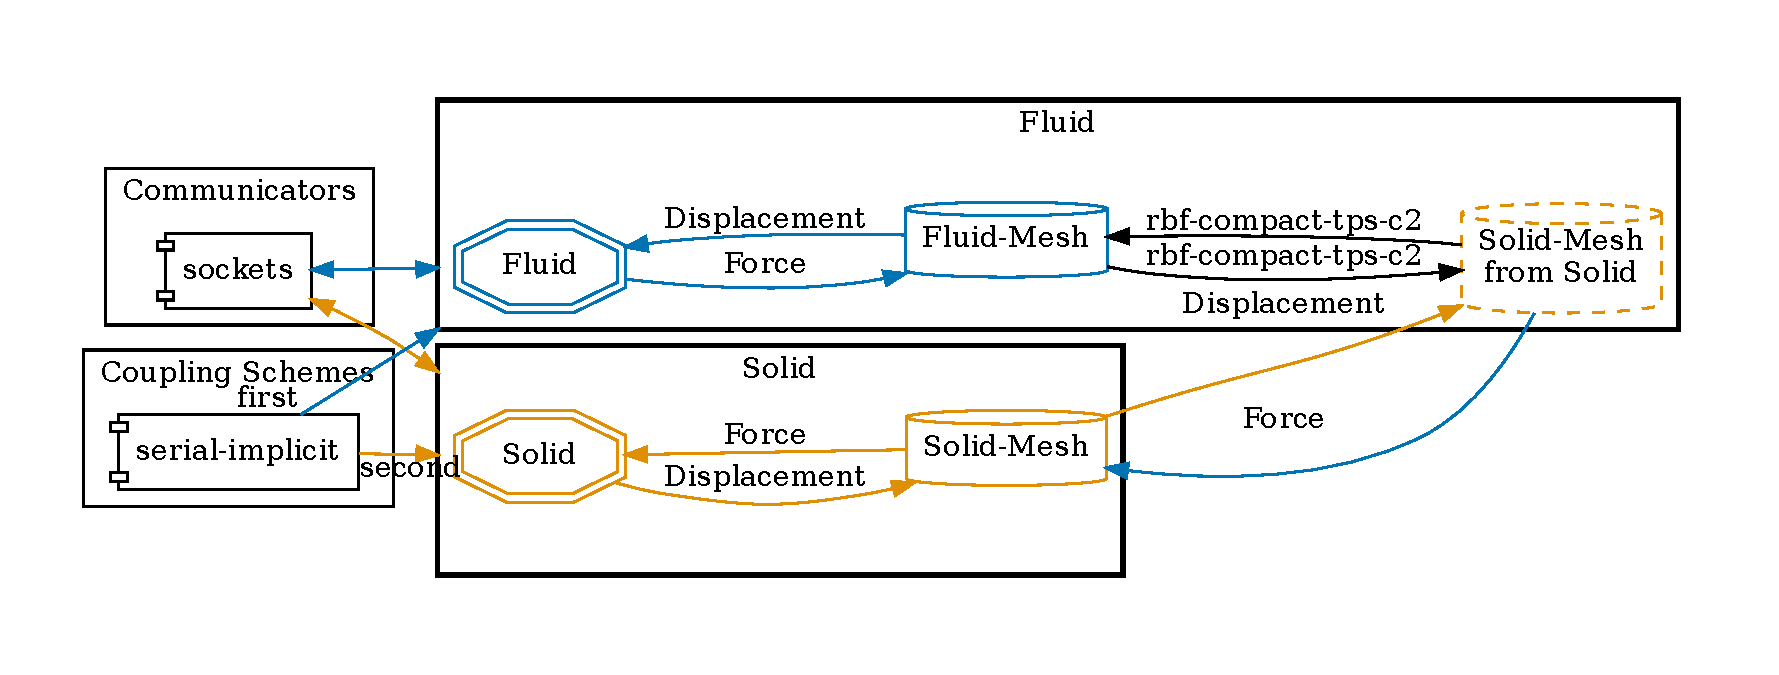
\includegraphics[width=\textwidth]{figs/precice-config.pdf}
\caption{
\label{fig:config}
Auto-generated visualization of the preCICE configuration of \autoref{code:config} using the \textit{Config Visualizer} of preCICE.}
\end{figure}


\paragraph{Coupling flow} The actual coupling between participants happens within the single preCICE API function \inpython{advance}, line 34 in \autoref{code:example}. This includes communication, mapping, and acceleration of coupling data -- whatever methods are defined in the preCICE configuration. To better understand the order and relation of individual coupling steps, \autoref{fig:schedule} depicts the overall coupling flow when using the example configuration of \autoref{code:config}.
For this visualization, we further assume that both participants use identical time step sizes.
During the initialization, \incode{Solid-Mesh} is sent from \incode{Solid} to \incode{Fluid}. 
A serial coupling scheme leads to a staggered execution of both participants: one after the other. This implies, in particular, that the behavior of both participants within the preCICE API functions cannot be symmetric.
In the example, \incode{Fluid} is the first participant of the coupling scheme. 
This means that, after the first time step of \incode{Fluid}, the first \inpython{advance} sends force values to \incode{Solid}, as can be seen in the figure. This coupling data is, however, already received in \inpython{initialize} of \incode{Solid}, such that the solver can use it in its first time step. The first displacement values are then sent at the start of the first \inpython{advance} of \incode{Solid} and received at the end of the first advance of \incode{Fluid}.  
Data is mapped in both direction within \inpython{advance} of \incode{Fluid}. Convergence acceleration of the coupling iteration is always executed in \inpython{advance} of the second participant, here \incode{Solid}.
Please note that a different preCICE configuration could lead to a completely different order and relation of steps: the roles of first and second could be swapped, one or both data mappings could be computed on \incode{Solid}, or the serial coupling scheme could be replaced by a parallel one, to only name a few choices. All these changes can be configured at runtime. The adapted fluid code in \autoref{code:example} remains unchanged -- and would remain unchanged even if \incode{Solid} would be coupled with a third participant. 


\begin{figure}[h!]
\begin{tikzpicture}

 \coordinate (FE) at (0,0.25);
 \coordinate (SE) at (15,0.25);
 \coordinate (F0) at (0,14);
 \coordinate (S0) at (15,14);
 \draw (F0) circle (1.5pt);
 \draw (FE) circle (1.5pt);
 \draw (S0) circle (1.5pt);
 \draw (SE) circle (1.5pt);
 
 \node[right] at (F0) {\small \texttt{precice.Interface("{\normalsize\color{blue1}{Fluid}}", \ldots)}};
 \node[left] at (S0) {\small \texttt{precice.Interface("{\normalsize\color{my_orange}{Solid}}", \ldots)}};

\coordinate (F2) at (0,13.5);
\coordinate (S2) at (15,13.5);
\node[right] at (F2) {\small \texttt{{\color{my_orange}{interface}}.initialize()}};
\node[left] at (S2) {\small \texttt{{\color{my_orange}{interface}}.initialize()}};
\draw (F2) circle (1.5pt);
\draw (S2) circle (1.5pt);

\coordinate (F_mesh) at (5.5,12.75);
\node[left] at (F_mesh) {\small receive mesh};
\coordinate (S_mesh) at (9.5,12.75);
\node[right] at (S_mesh) {\small send mesh};
\draw[->,thick] (S_mesh) -- (F_mesh) node[midway,above] {\small \color{my_orange} Solid-Mesh};


\coordinate (F3) at (0,12);
\coordinate (S3) at (15,9);
\node[right] at (F3) {\small \texttt{solve\_time\_step(\ldots)}};
\node[left] at (S3) {\small \texttt{solve\_time\_step(\ldots)}};
\draw (F3) circle (1.5pt);
\draw (S3) circle (1.5pt);

\coordinate (F4) at (0,11.5);
\coordinate (S4) at (15,8.5);
\node[right] at (F4) {\small \texttt{{\color{my_orange}{interface}}.advance()}};
\node[left] at (S4) {\small \texttt{{\color{my_orange}{interface}}.advance()}};
\draw (F4) circle (1.5pt);
\draw (S4) circle (1.5pt);

\coordinate (F_map1) at (2.5,10.5);
\node[left] at (F_map1) {\small \color{blue1} Fluid-Mesh};
\coordinate (F_map2) at (4.5,10.5);
\node[right] at (F_map2) {\small \color{my_orange} Solid-Mesh};
\draw[->, thick, densely dashed] (F_map1) -- (F_map2) node[midway,above] {\small map write data} node[midway,below] {\small Force};

\draw[|-|, dotted] (12,12.75) to node[midway,right] {\small \textit{waiting}} (12,9.75);


\coordinate (F_com1) at (5.5,9.75);
\node[left] at (F_com1) {\small send data};
\coordinate (S_com1) at (9.5,9.75);
\node[right] at (S_com1) {\small receive data};
\draw[->,thick,out=0,in=180] (F_com1) to node[midway,above] {\small  Force} (S_com1);


\coordinate (F_com2) at (5.5,7.25);
\node[left] at (F_com2) {\small receive data};
\coordinate (S_com2) at (9.5,7.25);
\node[right] at (S_com2) {\small send data};
\draw[->,thick, out=180,in=0] (S_com2) to node[midway,above] {\small   Displacement} (F_com2);

\draw[|-|, dotted] (3,9.75) to node[midway,left] {\small \textit{waiting}} (3,7.25);


\node[right] at (9.5,7.75) {\small accelerate data};

\coordinate (F_map3) at (2.5,6.25);
\node[left] at (F_map3) {\small \color{blue1} Fluid-Mesh};
\coordinate (F_map4) at (4.5,6.25);
\node[right] at (F_map4) {\small \color{my_orange} Solid-Mesh};
\draw[->, thick, densely dashed] (F_map4) -- (F_map3) node[midway,above] {\small map read data} node[midway,below] {\small Displacement};

\coordinate (F5) at (0,5.25);
\coordinate (S5) at (15,2.25);
\node[right] at (F5) {\small  \texttt{solve\_time\_step(\ldots)}};
\node[left] at (S5) {\small \texttt{solve\_time\_step(\ldots)}};
\draw (F5) circle (1.5pt);
\draw (S5) circle (1.5pt);

\coordinate (F6) at (0,4.75);
\coordinate (S6) at (15,1.75);
\node[right] at (F6) {\small \texttt{{\color{my_orange}{interface}}.advance()}};
\node[left] at (S6) {\small \texttt{{\color{my_orange}{interface}}.advance()}};
\draw (F6) circle (1.5pt);
\draw (S6) circle (1.5pt);

\coordinate (F_map5) at (2.5,3.75);
\node[left] at (F_map5) {\small \color{blue1} Fluid-Mesh};
\coordinate (F_map6) at (4.5,3.75);
\node[right] at (F_map6) {\small \color{my_orange} Solid-Mesh};
\draw[->, thick, densely dashed] (F_map5) -- (F_map6) node[midway,above] {\small map write data} node[midway,below] {\small Force};

\coordinate (F_com3) at (5.5,3);
\node[left] at (F_com3) {\small send data};
\coordinate (S_com3) at (9.5,3);
\node[right] at (S_com3) {\small receive data};
\draw[->,thick,out=0,in=180] (F_com3) to node[midway,above] {\small   Force} (S_com3);

\draw[|-|, dotted] (12,7.25) to node[midway,right] {\small \textit{waiting}} (12,3);

\coordinate (F7) at (0,1.25);
\coordinate (S7) at (15,1.25);
\draw (F7) circle (1.5pt);
\draw (S7) circle (1.5pt);

\coordinate (F8) at (0,0.75);
\coordinate (S8) at (15,0.75);
\draw (F8) circle (1.5pt);
\draw (S8) circle (1.5pt);

\node[right] at (FE) {\small \texttt{{\color{my_orange}{interface}}.finalize()}};
\node[left] at (SE) {\small \texttt{{\color{my_orange}{interface}}.finalize()}};

\draw [->, shorten <=.1cm, shorten >=.1cm] (F0) to (F2);
\draw [->, shorten <=.1cm, shorten >=.1cm] (F2) to (F3);
\draw [->, shorten <=.1cm, shorten >=.1cm] (F3) to (F4);
\draw [->, shorten <=.1cm, shorten >=.1cm] (F4) to (F5);
\draw [->, shorten <=.1cm, shorten >=.1cm] (F5) to (F6);
\draw [->, shorten <=.1cm, shorten >=.1cm] (F6) to (F7);
\draw [dotted, shorten <=.1cm, shorten >=.1cm] (F7) to (F8);
\draw [->, shorten <=.1cm, shorten >=.1cm] (F8) to (FE);
\draw [->, shorten <=.1cm, shorten >=.1cm] (S0) to (S2);
\draw [->, shorten <=.1cm, shorten >=.1cm] (S2) to (S3);
\draw [->, shorten <=.1cm, shorten >=.1cm] (S3) to (S4);
\draw [->, shorten <=.1cm, shorten >=.1cm] (S4) to (S5);
\draw [->, shorten <=.1cm, shorten >=.1cm] (S5) to (S6);
\draw [->, shorten <=.1cm, shorten >=.1cm] (S6) to (S7);
\draw [dotted, shorten <=.1cm, shorten >=.1cm] (S7) to (S8);
\draw [->, shorten <=.1cm, shorten >=.1cm] (S8) to (SE);
\end{tikzpicture}
\caption{
\label{fig:schedule}
Overall flow of coupling steps resulting from the preCICE configuration of \autoref{code:config}.
The serial coupling scheme leads to a staggered execution of both participants, one after the other. Both participants wait in \inpython{initialize} and \inpython{advance} for synchronization. We assume identical time step sizes in both participants.
}
\end{figure}
  
\paragraph{Timestepping} So far, we assumed  that the coupled participants use matching time step sizes. preCICE is, however, also able to handle non-matching time step sizes. 
Then, data is only exchanged at the end of each time window, defined in the preCICE configuration, line 26 of \autoref{code:config}. Alternatively, the time window size can also be imposed by the first participant.
If a solver uses a smaller time step size than the time window size, it subcycles within the time window. This means, in particular, that the same coupling data is used throughout the time window, which can reduce the time discretization order of the coupled codes. We are currently working on a higher order time representation of coupling data to sample from, a coupling procedure known as waveform iteration~\cite{QNWI}.
To allow preCICE to track the time of a solver, the current time step size needs to be passed to preCICE in \incode{advance}, cf.~line 34 in \autoref{code:example}. preCICE then returns the remaining time within the current time window, which the coupled solver has to respect. Therefore, in line 27, the solver's time step size is restricted, if required. 



\paragraph{Implicit coupling}
We still need to explain how implicit coupling is realized. Please remember that by implicit coupling we mean the repetition of time windows until sufficient convergence of coupling data (cf.~\autoref{ssec:cplscheme}). To this end, a coupled solver needs to be able to move backwards in time, which we realize by writing and reading checkpoints of the complete internal solver state (lines 20 and 37 in \autoref{code:example}). Writing checkpoints is required when entering time windows for the first time and reading checkpoints is required at the end of a time window, whenever convergence is not achieved. As the solver does not know anything about the coupling scheme, preCICE tells the solver when it is time to write and read checkpoints in lines 19 and 36. At the end of the loop body, time is only increased when convergence is achieved, in line 40. Please note that, with this checkpointing mechanism, nested time and coupling loops are not necessary, but everything can be handled within one \incode{while} loop.


\paragraph{Help and further information}
We cannot explain all preCICE API functions and all configuration options with this single example. Please also consider the official user documentation\footnote{preCICE documentation: \url{https://precice.org/docs.html}}, which includes complete API and configuration references.
preCICE supports adapter development by extensive sanity checks of correct API usage -- a simple example: \texttt{advance} cannot be called before \inpython{initialize}. Moreover, the preCICE configuration is checked against the configuration reference and extensive logging is configurable.


